\lhead{Mobile-C API in the C/C++ Binary Space}
\noindent
The header file {\bf libmc.h} defines all the data types, macros 
and function prototypes for the Mobile-C library.
The header file is used in the C/C++ binary space.

\begin{table}[!h]
\capstart
\begin{center}
\caption{Data types defined in {\bf libmc.h}.}
\begin{tabular}{p{50 mm}p{110 mm}}
\hline
Data Type & Description \\
\hline
{\bf MCAgency\_t} & A handle containing information of an agency. \\
{\bf MCAgent\_t} & A handle containing information of a mobile agent. \\
{\bf MCAgencyOptions\_t} & A structure containing information about which thread(s) to be activated and the default agent status specified by a user. \\
\hline
\end{tabular}
\end{center}
\label{mobilec_datatype}
\end{table}

The header file {\bf fipa\_acl.h} contains datatype and macros related to 
FIPA ACL messaging, as described in Chapter \ref{chap:fipa}. This header
file may be used in both C/C++ binary space, as well as agent space.

\begin{table}[!h]
\capstart
\begin{center}
\caption{Data types defined in {\bf fipa\_acl.h}.}
\begin{tabular}{p{50 mm}p{110 mm}}
\hline
Data Type & Description \\
\hline
{\bf fipa\_acl\_message\_t} & A structure containing a FIPA ACL message. \\
\hline
\end{tabular}
\end{center}
\label{fipa_datatype}
\end{table}

\pagebreak

\begin{table}[!h]
\capstart
\begin{center}
\caption{Macros defined in {\bf libmc.h}.}
\begin{tabular}{p{50 mm}p{110 mm}}
\hline
Macro & Description \\
\hline
{\texttt enum MC\_ThreadIndex\_e} & \\
\hline
{\bf MC\_THREAD\_AI} \index{MC\_THREAD\_AI} & Identifier for agent initalizing thread. \\
{\bf MC\_THREAD\_AM} \index{MC\_THREAD\_AM} & Identifier for agent managing thread. \\
{\bf MC\_THREAD\_CL} \index{MC\_THREAD\_CL} & Identifier for connection listening thread. \\
{\bf MC\_THREAD\_MR} \index{MC\_THREAD\_MR} & Identifier for message receiving thread. \\
{\bf MC\_THREAD\_MS} \index{MC\_THREAD\_MS} & Identifier for message sending thread. \\
{\bf MC\_THREAD\_CP} \index{MC\_THREAD\_CP} & Identifier for command prompt thread. \\
{\bf MC\_THREAD\_ALL} \index{MC\_THREAD\_ALL} & Identifier for all threads. \\
\hline
{\texttt enum MC\_Signal\_e} & \\
\hline
{\bf MC\_RECV\_CONNECTION} \index{MC\_RECV\_CONNECTION} & Signal activated after an agency accepts a connection. \\
{\bf MC\_RECV\_MESSAGE} \index{MC\_RECV\_MESSAGE} & Signal activated after an agency receives an ACL message. \\
{\bf MC\_RECV\_AGENT} \index{MC\_RECV\_AGENT} & Signal activated after an agency receives a mobile agent. \\
{\bf MC\_RECV\_RETURN} \index{MC\_RECV\_RETURN} & Signal activated after an agency receives return data from a completed mobile agent. \\
{\bf MC\_EXEC\_AGENT} \index{MC\_EXEC\_AGENT} & Signal activated after a mobile agent is executed. \\
{\bf MC\_ALL\_SIGNALS} \index{MC\_ALL\_SIGNALS} & Signal activated after any of the above four events occurs. \\
\hline
{\texttt enum MC\_AgentType\_e} \index{MC\_AgentType\_e}& \\
\hline
{\bf MC\_REMOTE\_AGENT} \index{MC\_REMOTE\_AGENT} & Identifier for a remote mobile agent. \\
{\bf MC\_LOCAL\_AGENT} \index{MC\_LOCAL\_AGENT} & Identifier for a local mobile agent.\\
{\bf MC\_RETURN\_AGENT} \index{MC\_RETURN\_AGENT} & Identifier for a return mobile agent. \\
\hline
{\texttt enum MC\_AgentStatus\_e} \index{MC\_AgentStatus\_e} & \\
\hline
{\bf MC\_WAIT\_CH} \index{MC\_WAIT\_CH} & Value indicating a mobile agent is waiting to be executed. \\
{\bf MC\_WAIT\_MESSGSEND} \index{MC\_WAIT\_MESSGSEND}& Value indicating a mobile agent is waiting to be exported to another agency. \\
{\bf MC\_AGENT\_ACTIVE} \index{MC\_AGENT\_ACTIVE}& Value indicating a mobile agent is being executed. \\
{\bf MC\_AGENT\_NEUTRAL} \index{MC\_AGENT\_NEUTRAL}& Value indicating a mobile agent is waiting for an unspecified reason. \\
{\bf MC\_AGENT\_SUSPENDED} \index{MC\_AGENT\_SUSPENDED}& Value indicating a mobile agent is being suspended. \\
{\bf MC\_WAIT\_FINISHED} \index{MC\_WAIT\_FINISHED}& Value indicating a mobile agent has been executed and is waiting to be removed. \\
\hline
\end{tabular}
\end{center}
\label{mobilec_macro}
\end{table}

\begin{table}[!hp]
\capstart
\begin{center}
\caption{Macros defined in {\bf fipa\_acl.h}. Detailed documentation for the
FIPA performatives and protocols may be found in the FIPA specifications at
\texttt{http://www.fipa.org}.}
\begin{tabular}{p{90 mm}p{70 mm}}
\hline
Macro & Description \\
\hline
{\texttt fipa\_performative\_e \index{fipa\_performative\_e}} & \\
\hline
{\bf FIPA\_ACCEPT\_PROPOSAL} \index{FIPA\_ACCEPT\_PROPOSAL} & The \texttt{accept-proposal} performative. \\
{\bf FIPA\_AGREE} \index{FIPA\_AGREE} & The \texttt{agree} performative. \\
{\bf FIPA\_CANCEL} \index{FIPA\_CANCEL} & The \texttt{cancel} performative. \\
{\bf FIPA\_CALL\_FOR\_PROPOSAL} \index{FIPA\_CALL\_FOR\_PROPOSAL} & The \texttt{call-for-proposal} performative. \\
{\bf FIPA\_CONFIRM} \index{FIPA\_CONFIRM} & The \texttt{confirm} performative. \\
{\bf FIPA\_DISCONFIRM} \index{FIPA\_DISCONFIRM} & The \texttt{disconfirm} performative. \\
{\bf FIPA\_FAILURE} \index{FIPA\_FAILURE} & The \texttt{failure} performative. \\
{\bf FIPA\_INFORM} \index{FIPA\_INFORM} & The \texttt{inform} performative. \\
{\bf FIPA\_INFORM\_IF} \index{FIPA\_INFORM\_IF} & The \texttt{inform-if} performative. \\
{\bf FIPA\_INFORM\_REF} \index{FIPA\_INFORM\_REF} & The \texttt{inform-ref} performative. \\
{\bf FIPA\_NOT\_UNDERSTOOD} \index{FIPA\_NOT\_UNDERSTOOD} & The \texttt{not-understood} performative. \\
{\bf FIPA\_PROPOGATE} \index{FIPA\_PROPOGATE} & The \texttt{propogate} performative. \\
{\bf FIPA\_PROPOSE} \index{FIPA\_PROPOSE} & The \texttt{propose} performative. \\
{\bf FIPA\_PROXY} \index{FIPA\_PROXY} & The \texttt{proxy} performative. \\
{\bf FIPA\_QUERY\_IF} \index{FIPA\_QUERY\_IF} & The \texttt{query-if} performative. \\
{\bf FIPA\_QUERY\_REF} \index{FIPA\_QUERY\_REF} & The \texttt{query-ref} performative. \\
{\bf FIPA\_REFUSE} \index{FIPA\_REFUSE} & The \texttt{refuse} performative. \\
{\bf FIPA\_REJECT\_PROPOSAL} \index{FIPA\_REJECT\_PROPOSAL} & The \texttt{reject-proposal} performative. \\
{\bf FIPA\_REQUEST} \index{FIPA\_REQUEST} & The \texttt{request} performative. \\
{\bf FIPA\_REQUEST\_WHEN} \index{FIPA\_REQUEST\_WHEN} & The \texttt{request-when} performative. \\
{\bf FIPA\_REQUEST\_WHENEVER} \index{FIPA\_REQUEST\_WHENEVER} & The \texttt{request-whenever} performative. \\
{\bf FIPA\_SUBSCRIBE} \index{FIPA\_SUBSCRIBE} & The \texttt{subscribe} performative. \\
\hline
{\texttt enum fipa\_protocol\_e} & \\
\hline
{\bf FIPA\_PROTOCOL\_REQUEST} \index{FIPA\_PROTOCOL\_REQUEST} & The FIPA \texttt{request} protocol. \\
{\bf FIPA\_PROTOCOL\_QUERY} \index{FIPA\_PROTOCOL\_QUERY} & The FIPA \texttt{query} protocol. \\
{\bf FIPA\_PROTOCOL\_REQUEST\_WHEN} \index{FIPA\_PROTOCOL\_REQUEST\_WHEN} & The FIPA \texttt{request-when} protocol. \\
{\bf FIPA\_PROTOCOL\_CONTRACT\_NET} \index{FIPA\_PROTOCOL\_CONTRACT\_NET} & The FIPA \texttt{contract-net} protocol. \\
{\bf FIPA\_PROTOCOL\_ITERATED\_CONTRACT\_NET} \index{FIPA\_PROTOCOL\_ITERATED\_CONTRACT\_NET} & The FIPA \texttt{iterated-contract-net} protocol. \\
{\bf FIPA\_PROTOCOL\_ENGLISH\_AUCTION} \index{FIPA\_PROTOCOL\_ENGLISH\_AUCTION} & The FIPA \texttt{english-auction} protocol. \\
{\bf FIPA\_PROTOCOL\_DUTCH\_AUCTION} \index{FIPA\_PROTOCOL\_DUTCH\_AUCTION} & The FIPA \texttt{dutch-auction} protocol. \\
{\bf FIPA\_PROTOCOL\_BROKERING} \index{FIPA\_PROTOCOL\_BROKERING} & The FIPA \texttt{brokering} protocol. \\
{\bf FIPA\_PROTOCOL\_RECRUITING} \index{FIPA\_PROTOCOL\_RECRUITING} & The FIPA \texttt{recruiting} protocol. \\
{\bf FIPA\_PROTOCOL\_SUBSCRIBE} \index{FIPA\_PROTOCOL\_SUBSCRIBE} & The FIPA \texttt{subscribe} protocol. \\
{\bf FIPA\_PROTOCOL\_PROPOSE} \index{FIPA\_PROTOCOL\_PROPOSE} & The FIPA \texttt{propose} protocol. \\
{\bf FIPA\_PROTOCOL\_END} \index{FIPA\_PROTOCOL\_END} & The FIPA \texttt{end} protocol. \\
\hline
\end{tabular}
\end{center}
\label{fipa_macro}
\end{table}

\begin{table}[!hp]
\capstart
\begin{center}
\caption{Functions in the C/C++ binary space.}
\begin{tabular}{p{78 mm}p{77 mm}}
%\begin{tabular}{ll}
\hline
Function & Description \\
\hline
{\bf MC\_AclAddReceiver()} \dotfill & Add a receiver to an ACL message. \\
{\bf MC\_AclAddReplyTo()} \dotfill & Add a reply-to address to an ACL message. \\
{\bf MC\_AclGetContent()} \dotfill & Get the content of an ACL message. \\
{\bf MC\_AclGetConversationID()} \dotfill & Get the conversation id from an ACL message. \\
{\bf MC\_AclGetPerformative()} \dotfill & Get the performative of an ACL message. \\
{\bf MC\_AclGetProtocol()} \dotfill & Get the protocol from an ACL message. \\
{\bf MC\_AclGetSender()} \dotfill & Get the sender of an ACL message. \\
{\bf MC\_AclNew()} \dotfill & Allocate a new FIPA ACL message. \\
{\bf MC\_AclPost()} \dotfill & Post a FIPA ACL message to an agent's mailbox. \\
{\bf MC\_AclReply()} \dotfill & Allocate a new FIPA ACL message automatically addressed to the sender of a previous message. \\
{\bf MC\_AclRetrieve()} \dotfill & Retrieve an ACL message from an agent's mailbox. \\
{\bf MC\_AclSetContent()} \dotfill & Set the content of an ACL message. \\
{\bf MC\_AclSetConversationID()} \dotfill & Set the conversation id of an ACL message. \\
{\bf MC\_AclSetPerformative()} \dotfill & Set the performative of an ACL message. \\
{\bf MC\_AclSetProtocol()} \dotfill & Set the protocol of an ACL message. \\
{\bf MC\_AclSetSender()} \dotfill & Set the sender of an ACL message. \\
{\bf MC\_AclWaitRetrieve()} \dotfill & Wait for a message to arrive at an agent's mailbox. \\
{\bf MC\_AgentAddTask()} \dotfill & Add a task to an agent based off of C source code. \\
{\bf MC\_AgentAddTaskFromFile()} \dotfill & Add a task to an agent based off of a C source code file. \\
{\bf MC\_AgentAttachFile()} \dotfill & Attach a file to the agent's current task. \\
{\bf MC\_AgentListFiles()} \dotfill & List files attached to an agent's task. \\
{\bf MC\_AgentRetrieveFile()} \dotfill & Retrieve and save an agent's attached file onto the filesystem. \\
{\bf MC\_AgentReturnArrayDim()} \dotfill & Get the dimension of an array returned by an agent. \\
{\bf MC\_AgentReturnArrayExtent()} \dotfill & Get the extent of a dimension of an array returned by an agent. \\
{\bf MC\_AgentReturnArrayNum()} \dotfill & Get the number of elements of an array returned by an agent. \\
{\bf MC\_AgentReturnDataGetSymbolAddr()} \dotfill & Get a pointer to an array returned by an agent. \\
{\bf MC\_AgentReturnDataSize()} \dotfill & Get the size of a single element of the array. \\
{\bf MC\_AgentReturnDataType()} \dotfill & Get the type of the array. \\
{\bf MC\_AgentReturnIsArray()} \dotfill & Determine if the returned variable is an array. \\
{\bf MC\_AddAgent()} \dotfill & Add a mobile agent into an agency. \\
{\bf MC\_AddAgentInitCallback()} \dotfill & Add an agent initialization callback function into an agency. \\
{\bf MC\_AddStationaryAgent()} \dotfill & Add a mobile agent into an agency. \\
%{\bf MC\_AgentVariableRetrieve()} & Retrieve a saved variable from an agent's prior task. \\
%{\bf MC\_AgentVariableSave()} & Save an agent's task variable for migration. \\
{\bf MC\_Barrier()} \dotfill & Block until all agents in an agency have called this function. \\
{\bf MC\_BarrierDelete()} \dotfill & Delete a Mobile-C barrier. \\
{\bf MC\_BarrierInit()} \dotfill & Initialize a Mobile-C barrier. \\
{\bf MC\_CallAgentFunc()} \dotfill & Call a function defined in an agent. \\
{\bf MC\_CallAgentFuncV()} \dotfill & Call a function defined in an agent. \\
\hline
\end{tabular}
\end{center}
\label{mobilec_api_cbinary}
\end{table}

\addtocounter{table}{-1}
\begin{table}[!hp]
\capstart
\begin{center}
\caption{Functions in the C/C++ binary space (contd.).}
%\begin{tabular}{ll}
\begin{tabular}{p{78 mm}p{77 mm}}
\hline
Function & Description \\
\hline
{\bf MC\_CallAgentFuncVar()} \dotfill & Call a function defined in an agent. \\
{\bf MC\_ChInitializeOptions()} \dotfill & Set the initialization options for a Ch to be used as one AEE in an agency. \\
{\bf MC\_ComposeAgent()} \dotfill & Compose an agent from program source code. \\
{\bf MC\_ComposeAgentS()} \dotfill & [Deprecated] Compose an agent from program source code with a workgroup code. \\
{\bf MC\_ComposeAgentWithWorkgroup()} \dotfill & Compose an agent from program source code with a workgroup code. \\
{\bf MC\_ComposeAgentFromFile()} \dotfill & Compose an agent from a program source code file. \\
{\bf MC\_ComposeAgentFromFileS()} \dotfill & [Deprecated] Compose an agent from a program source code file with a workgroup code. \\
{\bf MC\_ComposeAgentFromFileWithWorkgroup()} & Compose an agent from a program source code file with a workgroup code. \\
{\bf MC\_CondBroadcast()} \dotfill & Wake up all agents/threads waiting on a condition variable. \\
{\bf MC\_CondReset()} \dotfill & Reset a Mobile-C condition variable. \\
{\bf MC\_CondSignal()} \dotfill & Signal another agent that is waiting on a condition variable. \\
{\bf MC\_CondWait()} \dotfill & Cause the calling agent or thread to wait on a Mobile-C condition variable with the ID specified by the argument. \\
{\bf MC\_CopyAgent()} \dotfill & Perform a deep copy to copy an agent. \\
{\bf MC\_DeleteAgent()} \dotfill & Stop and remove an agent from an agency. \\
{\bf MC\_DeregisterService()} \dotfill & Deregister a service with the Directory Facilitator. \\
{\bf MC\_End()} \dotfill & Terminate a Mobile-C agency. \\
{\bf MC\_FindAgentByID()} \dotfill & Find a mobile agent by its ID number in an agency.\\
{\bf MC\_FindAgentByName()} \dotfill & Find a mobile agent by its name in an agency. \\
{\bf MC\_GetAgentArrivalTime()} \dotfill & Get the time when an agent arrives an agency. \\
{\bf MC\_GetAgentExecEngine()} \dotfill & Get the AEE associated with a mobile agent in an agency. \\
{\bf MC\_GetAgentID()} \dotfill & Get the ID of an agent. \\
{\bf MC\_GetAgentName()} \dotfill & Get the name of an agent. \\
{\bf MC\_GetAgentNumTasks()} \dotfill & Get the number of tasks a mobile agent has. \\
{\bf MC\_GetAgentReturnData()} \dotfill & [Deprecated] Get the return data of a mobile agent. \\
{\bf MC\_GetAgentStatus()} \dotfill & Get the status of a mobile agent in an agency. \\
{\bf MC\_GetAgentType()} \dotfill & Get the type of a mobile agent. \\
{\bf MC\_GetAgentXMLString()} \dotfill & Retrieve a mobile agent message in XML format as a character string. \\
{\bf MC\_GetAllAgents()} \dotfill & Obtain all the agents in an agency. \\
{\bf MC\_HaltAgency()} \dotfill & Halt an agency's operation. \\
{\bf MC\_Initialize()} \dotfill & Start a Mobile-C agency and return a handle of the launched agency. \\
{\bf MC\_InitializeAgencyOptions()} \dotfill & Initialize Mobile-C options. \\
{\bf MC\_LoadAgentFromFile()} \dotfill & Load an agent from an XML file into a local agency.\\
\hline
\end{tabular}
\end{center}
\end{table}
\pagebreak

\addtocounter{table}{-1}
\begin{table}[!hp]
\capstart
\begin{center}
\caption{Functions in the C/C++ binary space (contd.).}
%\begin{tabular}{ll}
\begin{tabular}{p{63 mm}p{97 mm}}
\hline
Function & Description \\
\hline
{\bf MC\_MainLoop()} \dotfill & Cause the calling thread to wait indefinitely on an agency.\\
{\bf MC\_MigrateAgent()} \dotfill & Migrate an agent. \\
{\bf MC\_MutexLock()} \dotfill & Lock a previously initialized Mobile-C synchronization variable as a mutex. \\
{\bf MC\_MutexUnlock()} \dotfill & Unlock a locked Mobile-C synchronization variable. \\
{\bf MC\_PrintAgentCode()} \dotfill & Print a mobile agent code for inspection. \\
{\bf MC\_RegisterService()} \dotfill &  Register a new service with the Directory Facilitator. \\
{\bf MC\_ResetSignal()} \dotfill &  Reset the Mobile-C signalling system. \\
{\bf MC\_ResumeAgency()} \dotfill &  Resume an agency's operation. \\
{\bf MC\_RetrieveAgent()} \dotfill & Retrieve the first neutral mobile agent from a mobile agent list. \\
{\bf MC\_RetrieveAgentCode()} \dotfill & Retrieve a mobile agent code in the form of a character string. \\
{\bf MC\_SearchForService()} \dotfill & Search the Directory Facilitator for a service. \\
{\bf MC\_SemaphorePost()} \dotfill & Unlock one resource from a Mobile-C semaphore. \\
{\bf MC\_SemaphoreWait()} \dotfill & Allocate one resource from a Mobile-C synchronization semaphore variable. \\
{\bf MC\_SendAgent()} \dotfill & Send an ACL mobile agent message to a remote agency. \\
{\bf MC\_SendAgentFile()} \dotfill & Send an ACL mobile agent message saved as a file to a remote agency. \\
{\bf MC\_SendAgentMigrationMessage()} \dotfill & [Deprecated] Send an ACL mobile agent message to a remote agency. \\
{\bf MC\_SendAgentMigrationMessageFile()} \dotfill & [Deprecated] Send an ACL mobile agent message saved as a file to a remote agency. \\
{\bf MC\_SendSteerCommand()} \dotfill & Send a command to control a steerable binary space function. \\
{\bf MC\_SetAgentStatus()} \dotfill & Set the status of a mobile agent in an agency. \\
{\bf MC\_SetDefaultAgentStatus()} \dotfill & Assign a user defined default status to all incoming mobile agents. \\
{\bf MC\_SetThreadOff()} \dotfill & Deactivate a thread in an agency. \\
{\bf MC\_SetThreadOn()} \dotfill & Activate a thread in an agency. \\
{\bf MC\_Steer()} \dotfill & Set up a steerable binary space function. \\
{\bf MC\_SteerControl()} \dotfill & Retrieve a steering command from the mobile agent space. \\
{\bf MC\_SyncDelete()} \dotfill & Delete a previously initialized synchronization variable. \\
{\bf MC\_SyncInit()} \dotfill & Initialize a new synchronization variable. \\
{\bf MC\_TerminateAgent()} \dotfill & Terminate the execution of a mobile agent in an agency. \\
%{\bf MC\_Wait()} \dotfill & Cause the calling thread to wait indefinitely on an agency.\\
{\bf MC\_WaitAgent()} \dotfill & Cause the calling thread to wait until a mobile agent is received. \\
{\bf MC\_WaitRetrieveAgent()} \dotfill & Block the calling thread until a mobile agent arrives, and return the mobile agent instead of executing it. \\
{\bf MC\_WaitSignal()} \dotfill & Block until one of the signals in the second argument is signalled.\\
\hline
\end{tabular}
\end{center}
\end{table}
\pagebreak

\newpage
\input{api/MC_AclGetProtocol}
\pagebreak
\rhead{\bf MC\_AclAddReceiver()}
\noindent
\vspace{5pt}
\rule{6.5in}{0.015in}
\noindent
\phantomsection
{\LARGE \bf MC\_AclAddReceiver()\index{MC\_AclAddReceiver()}}\\
\addcontentsline{toc}{section}{MC\_AclAddReceiver()}
\label{api:MC_Acl_AddReceiver()}

\noindent
{\bf Synopsis}\\
{\bf \#include $<$libmc.h$>$}\\
{\bf int MC\_AclAddReceiver}({\bf fipa\_acl\_message\_t*} acl, {\bf const char*} name, {\bf const char*} address );\\

\noindent
{\bf Purpose}\\
Add a receiver to the ACL message.\\

\noindent
{\bf Return Value}\\
Returns 0 on success or non-zero on failure.

\noindent
{\bf Parameters}
\vspace{-0.1in}
\begin{description}
\item
\begin{tabular}{p{10 mm}p{145 mm}} 
$acl$ & An initialized ACL message. \\
$name$ & Sets the name of the receiver. \\
$address$ & Sets the address of the receiver. 
\end{tabular}
\end{description}

\noindent
{\bf Description}\\
This function is used to add a receiver to an ACL message. This function 
may be called multiple times on an ACL message. each time this function is 
called, a new receiver is appended to the list of intended receivers
for the ACL message. \\

\noindent
{\bf Example}\\
\noindent
{\footnotesize\verbatiminput{../demos/FIPA_compliant_ACL_messages/fipa_test/test2.xml}}

\noindent
{\bf See Also}\\
\texttt{
  MC\_AclSetPerformative(), MC\_AclSetSender(), MC\_AclAddReplyTo(), 
\linebreak MC\_AclSetContent()}


%\CPlot::\DataThreeD(), \CPlot::\DataFile(), \CPlot::\Plotting(), \plotxy().\\

\pagebreak
\rhead{\bf MC\_AclAddReplyTo()}
\noindent
\vspace{5pt}
\rule{6.5in}{0.015in}
\noindent
\phantomsection
{\LARGE \bf MC\_AclAddReplyTo()\index{MC\_AclAddReplyTo()}}\\
\addcontentsline{toc}{section}{MC\_AclAddReplyTo()}
\label{api:MC_Acl_AddReplyTo()}

\noindent
{\bf Synopsis}\\
{\bf \#include $<$libmc.h$>$}\\
{\bf int MC\_AclAddReplyTo}({\bf fipa\_acl\_message\_t*} acl, {\bf const char*} name, {\bf const char*} address );\\

\noindent
{\bf Purpose}\\
Add a reply-to address to the ACL message.\\

\noindent
{\bf Return Value}\\
Returns 0 on success or non-zero on failure. \\

\noindent
{\bf Parameters}
\vspace{-0.1in}
\begin{description}
\item
\begin{tabular}{p{10 mm}p{145 mm}} 
$acl$ & An initialized ACL message. \\
$name$ & Sets the name of the reply-to destination. \\
$address$ & Sets the address of the reply-to destination. 
\end{tabular}
\end{description}

\noindent
{\bf Description}\\
This function is used to add a reply-to address to an ACL message. This function 
may be called multiple times on an ACL message. each time this function is 
called, a new reply-to address is appended to the list of intended reply-to
addresses for the ACL message. \\

\noindent
{\bf Example}\\
\noindent
{\footnotesize\verbatiminput{../demos/FIPA_compliant_ACL_messages/fipa_test/test2.xml}}

\noindent
{\bf See Also}\\
\texttt{
  MC\_AclSetPerformative(), MC\_AclSetSender(), MC\_AclAddReceiver(), \linebreak
    MC\_AclSetContent()
}

%\CPlot::\DataThreeD(), \CPlot::\DataFile(), \CPlot::\Plotting(), \plotxy().\\

\pagebreak
\rhead{\bf MC\_AclGetContent()}
\noindent
\vspace{5pt}
\rule{6.5in}{0.015in}
\noindent
\phantomsection
{\LARGE \bf MC\_AclGetContent()\index{MC\_AclGetContent()}}\\
\addcontentsline{toc}{section}{MC\_AclGetContent()}
\label{api:MC_Acl_GetContent()}

\noindent
{\bf Synopsis}\\
{\bf \#include $<$libmc.h$>$}\\
{\bf const char* MC\_AclGetContent}({\bf fipa\_acl\_message\_t*} acl);\\

\noindent
{\bf Purpose}\\
Get the content of an ACL message.\\

\noindent
{\bf Return Value}\\
Returns a valid character string or NULL on failure. \\

\noindent
{\bf Parameters}
\vspace{-0.1in}
\begin{description}
\item
\begin{tabular}{p{10 mm}p{145 mm}} 
$acl$ & An initialized ACL message. \\
\end{tabular}
\end{description}

\noindent
{\bf Description}\\
This function gets the ``content'' field of an ACL message. \\

\noindent
{\bf Example}\\
\noindent
{\footnotesize\verbatiminput{../demos/FIPA_compliant_ACL_messages/fipa_test/test2.xml}}

\noindent
{\bf See Also}\\
\texttt{
  MC\_AclSetPerformative(), MC\_AclSetSender(), MC\_AclAddReceiver(), 
    \linebreak MC\_AclAddReplyTo()
}

%\CPlot::\DataThreeD(), \CPlot::\DataFile(), \CPlot::\Plotting(), \plotxy().\\

\pagebreak
\rhead{\bf MC\_AclGetConversationID()}
\noindent
\vspace{5pt}
\rule{6.5in}{0.015in}
\noindent
\phantomsection
{\LARGE \bf MC\_AclGetConversationID()\index{MC\_AclGetConversationID()}}\\
\addcontentsline{toc}{section}{MC\_AclGetConversationID()}
\label{api:MC_Acl_GetConversationID()}

\noindent
{\bf Synopsis}\\
{\bf \#include $<$libmc.h$>$}\\
{\bf const char* MC\_AclGetConversationID}({\bf fipa\_acl\_message\_t*} acl);\\

\noindent
{\bf Purpose}\\
Get the conversation id of an ACL message.\\

\noindent
{\bf Return Value}\\
Returns a character string on success of NULL on failure.\\

\noindent
{\bf Parameters}
\vspace{-0.1in}
\begin{description}
\item
\begin{tabular}{p{10 mm}p{145 mm}} 
$acl$ & An initialized ACL message. 
\end{tabular}
\end{description}

\noindent
{\bf Description}\\
This function gets the ``conversation-id'' field from an ACL message. 
The conversation ID is used to differentiate multiple agent conversations which
may be happening simultaneously between two agents. For more details, please
consult the FIPA specifications at \texttt{http://www.fipa.org}.\\

\noindent
{\bf See Also}\\
\texttt{
  MC\_AclSetPerformative(), MC\_AclSetSender(), MC\_AclAddReceiver(), 
    \linebreak MC\_AclAddReplyTo()
}

%\CPlot::\DataThreeD(), \CPlot::\DataFile(), \CPlot::\Plotting(), \plotxy().\\

\pagebreak
\rhead{\bf MC\_AclGetPerformative()}
\noindent
\vspace{5pt}
\rule{6.5in}{0.015in}
\noindent
\phantomsection
{\LARGE \bf MC\_AclGetPerformative()\index{MC\_AclGetPerformative()}}\\
\addcontentsline{toc}{section}{MC\_AclGetPerformative()}
\label{api:MC_Acl_GetPerformative()}

\noindent
{\bf Synopsis}\\
{\bf \#include $<$libmc.h$>$}\\
{\bf enum fipa\_performative\_e MC\_AclGetPerformative}({\bf fipa\_acl\_message\_t*} acl);\\

\noindent
{\bf Purpose}\\
Get the performative from an ACL message.\\

\noindent
{\bf Return Value}\\
Returns a valid FIPA performative enumeration or -1 on failure.

\noindent
{\bf Parameters}
\vspace{-0.1in}
\begin{description}
\item
\begin{tabular}{p{10 mm}p{145 mm}} 
$acl$ & An initialized ACL message. \\
\end{tabular}
\end{description}

\noindent
{\bf Description}\\
This function is used to get the FIPA ACL performative from an ACL message. 
The performative may be any valid FIPA performative listed in the table 
below. \\
\begin{tabular}{ll}
Enumerated Value & FIPA Perfomative \\ \hline
\texttt{FIPA\_ACCEPT\_PROPOSAL} & accept-proposal \\
\texttt{FIPA\_AGREE} & agree \\
\texttt{FIPA\_CANCEL} & cancel\\
\texttt{FIPA\_CALL\_FOR\_PROPOSAL} & call-for-proposal \\
\texttt{FIPA\_CONFIRM} & confirm\\
\texttt{FIPA\_DISCONFIRM} & disconfirm \\
\texttt{FIPA\_FAILURE} & failure \\
\texttt{FIPA\_INFORM} & inform \\
\texttt{FIPA\_INFORM\_IF} & inform-if \\
\texttt{FIPA\_INFORM\_REF} & inform-ref \\
\texttt{FIPA\_NOT\_UNDERSTOOD} & not-understood \\
\texttt{FIPA\_PROPOGATE} & propogate \\
\texttt{FIPA\_PROPOSE} & propose \\
\texttt{FIPA\_PROXY} & proxy \\
\texttt{FIPA\_QUERY\_IF} & query-if \\
\texttt{FIPA\_QUERY\_REF} & query-ref \\
\texttt{FIPA\_REFUSE} & refuse \\
\texttt{FIPA\_REJECT\_PROPOSAL} & reject-proposal \\
\texttt{FIPA\_REQUEST} & request \\
\texttt{FIPA\_REQUEST\_WHEN} & request-when \\
\texttt{FIPA\_REQUEST\_WHENEVER} & request-whenever \\
\texttt{FIPA\_SUBSCRIBE} & subscribe
\end{tabular}


\noindent
{\bf Example}\\
\noindent
{\footnotesize\verbatiminput{../demos/FIPA_compliant_ACL_messages/fipa_test/test2.xml}}

\noindent
{\bf See Also}\\
\texttt{
  MC\_AclSetSender(), MC\_AclAddReceiver(), MC\_AclAddReplyTo(), \linebreak 
    MC\_AclSetContent()
}

%\CPlot::\DataThreeD(), \CPlot::\DataFile(), \CPlot::\Plotting(), \plotxy().\\

\pagebreak
\input{api/MC_AclGetProtocol}
\pagebreak
\rhead{\bf MC\_AclGetSender()}
\noindent
\vspace{5pt}
\rule{6.5in}{0.015in}
\noindent
\phantomsection
{\LARGE \bf MC\_AclGetSender()\index{MC\_AclGetSender()}}\\
\addcontentsline{toc}{section}{MC\_AclGetSender()}
\label{api:MC_Acl_GetSender()}

\noindent
{\bf Synopsis}\\
{\bf \#include $<$libmc.h$>$}\\
{\bf int MC\_AclGetSender}({\bf fipa\_acl\_message\_t*} acl, {\bf char**} name, {\bf char**} address );\\

\noindent
{\bf Purpose}\\
Get the sender from an ACL message.\\

\noindent
{\bf Return Value}\\
Returns 0 on success or non-zero on failure.

\noindent
{\bf Parameters}
\vspace{-0.1in}
\begin{description}
\item
\begin{tabular}{p{10 mm}p{145 mm}} 
$acl$ & An initialized ACL message. \\
$name$ & (Output) Gets the name of the sender. \\
$address$ & (Output) Gets the address of the sender. 
\end{tabular}
\end{description}

\noindent
{\bf Description}\\
This function takes pointers to characters, automatically allocates space for
character strings, and makes copies of the names and addresses of an ACL message
onto those strings. The variables passed into the \texttt{name} and \texttt{address}
parameters of the function should be freed manually by the caller.

\noindent
{\bf Example}\\
\noindent
{\footnotesize\verbatiminput{../demos/FIPA_compliant_ACL_messages/fipa_test/test2.xml}}

\noindent
{\bf See Also}\\
\texttt{
  MC\_AclSetPerformative(), MC\_AclAddReceiver(), MC\_AclAddReplyTo(), 
    \linebreak MC\_AclSetContent()
}

%\CPlot::\DataThreeD(), \CPlot::\DataFile(), \CPlot::\Plotting(), \plotxy().\\

\pagebreak
\rhead{\bf MC\_AclNew()}
\noindent
\vspace{5pt}
\rule{6.5in}{0.015in}
\noindent
\phantomsection
{\LARGE \bf MC\_AclNew()\index{MC\_AclNew()}}\\
\addcontentsline{toc}{section}{MC\_AclNew()}
\label{api:MC_AclNew()}

\noindent
{\bf Synopsis}\\
{\bf \#include $<$libmc.h$>$}\\
{\bf fipa\_acl\_message\_t* MC\_AclNew}({\bf void});\\

\noindent
{\bf Purpose}\\
Create a new, blank ACL message.\\

\noindent
{\bf Return Value}\\
Returns a newly allocated ACL message structure or NULL on failure.\\

\noindent
{\bf Parameters}
None.\\

\noindent
{\bf Description}\\
This function allocates and returns a new ACL message. All 
attributes of the message are set empty values and must be 
initialized before sending the message.\\

\noindent
{\bf Example}\\
\noindent
{\footnotesize\verbatiminput{../demos/FIPA_compliant_ACL_messages/fipa_test/test2.xml}}

\noindent
{\bf See Also}\\
\texttt{
  MC\_AclPost(), MC\_AclReply(), MC\_AclRetrieve(), MC\_AclSend(), \linebreak
    MC\_AclWaitRetrieve()
}

%\CPlot::\DataThreeD(), \CPlot::\DataFile(), \CPlot::\Plotting(), \plotxy().\\

\pagebreak
\rhead{\bf MC\_AclPost()}
\noindent
\vspace{5pt}
\rule{6.5in}{0.015in}
\noindent
\phantomsection
{\LARGE \bf MC\_AclPost()\index{MC\_AclPost()}}\\
\addcontentsline{toc}{section}{MC\_AclPost()}
\label{api:MC_AclPost()}

\noindent
{\bf Synopsis}\\
{\bf \#include $<$libmc.h$>$}\\
{\bf int MC\_AclPost}({\bf MCAgent\_t} agent, {\bf fipa\_acl\_message\_t*} message);\\

\noindent
{\bf Purpose}\\
Post a message directly to an agent's mailbox.\\

\noindent
{\bf Return Value}\\
Returns 0 on success, non-zero on failure.\\

\noindent
{\bf Parameters}
\vspace{-0.1in}
\begin{description}
\item
\begin{tabular}{p{10 mm}p{145 mm}} 
$agent$ & An initialized mobile agent. \\
$message$ & The ACL message to post. 
\end{tabular}
\end{description}

\noindent
{\bf Description}\\
This function is used to post an ACL message directly to an agent's 
mailbox. The agent must reside on the same agency as the caller.
No forwarding or checking of any fields of the ACL message is performed.\\

\noindent
{\bf Example}\\
\noindent

\noindent
{\bf See Also}\\
\texttt{
  MC\_AclNew(), MC\_AclReply(), MC\_AclRetrieve(), MC\_AclSend(), \linebreak 
    MC\_AclWaitRetrieve()
}

%\CPlot::\DataThreeD(), \CPlot::\DataFile(), \CPlot::\Plotting(), \plotxy().\\

\pagebreak
\rhead{\bf MC\_AclReply()}
\noindent
\vspace{5pt}
\rule{6.5in}{0.015in}
\noindent
\phantomsection
{\LARGE \bf MC\_AclReply()\index{MC\_AclNew()}}\\
\addcontentsline{toc}{section}{MC\_AclReply()}
\label{api:MC_AclReply()}

\noindent
{\bf Synopsis}\\
{\bf \#include $<$libmc.h$>$}\\
{\bf int MC\_AclReply}({\bf fipa\_acl\_message\_t*} acl\_message);\\

\noindent
{\bf Purpose}\\
Automatically generate an ACL message addressed to the sender of an
incoming ACL message..\\

\noindent
{\bf Return Value}\\
A newly allocated ACL message with the 'receiver' field initialized, or
NULL on failure.\\

\noindent
{\bf Parameters}
\vspace{-0.1in}
\begin{description}
\item
\begin{tabular}{p{10 mm}p{145 mm}} 
$acl\_message$ & The message to generate a reply to.
\end{tabular}
\end{description}

\noindent
{\bf Description}\\
This function is designed to make replying to received ACL messages easier.
The function automatically generates a new ACL message with the correct
destination address to reach the sender of the original message.\\

\noindent
{\bf Example}\\
\noindent

\noindent
{\bf See Also}\\
\texttt{
  MC\_AclNew(), MC\_AclPost(), MC\_AclRetrieve(), MC\_AclSend(), \linebreak 
    MC\_AclWaitRetrieve()
}

%\CPlot::\DataThreeD(), \CPlot::\DataFile(), \CPlot::\Plotting(), \plotxy().\\

\pagebreak
\rhead{\bf MC\_AclRetrieve()}
\noindent
\vspace{5pt}
\rule{6.5in}{0.015in}
\noindent
\phantomsection
{\LARGE \bf MC\_AclRetrieve()\index{MC\_AclNew()}}\\
\addcontentsline{toc}{section}{MC\_AclRetrieve()}
\label{api:MC_AclRetrieve()}

\noindent
{\bf Synopsis}\\
{\bf \#include $<$libmc.h$>$}\\
{\bf int MC\_AclRetrieve}({\bf MCAgent\_t} agent);\\

\noindent
{\bf Purpose}\\
Retrieve a message from an agent's mailbox.\\

\noindent
{\bf Return Value}\\
An ACL message on success, or NULL if no messages are in the 
mailbox.\\

\noindent
{\bf Parameters}
\vspace{-0.1in}
\begin{description}
\item
\begin{tabular}{p{10 mm}p{145 mm}} 
$agent$ & An initialized mobile agent.
\end{tabular}
\end{description}

\noindent
{\bf Description}\\
This function is used to retrieve a message from an agent's mailbox. The
message are retrieved in FIFO order. If there are no messages in the
mailbox, the function will return NULL.\\

\noindent
{\bf Example}\\
\noindent
{\footnotesize\verbatiminput{../demos/FIPA_compliant_ACL_messages/fipa_test/test1.xml}}

\noindent
{\bf See Also}\\
\texttt{
  MC\_AclNew(), MC\_AclPost(), MC\_AclReply(), MC\_AclSend(), \linebreak
    MC\_AclWaitRetrieve()
}

%\CPlot::\DataThreeD(), \CPlot::\DataFile(), \CPlot::\Plotting(), \plotxy().\\

\pagebreak
\rhead{\bf MC\_AclSetContent()}
\noindent
\vspace{5pt}
\rule{6.5in}{0.015in}
\noindent
\phantomsection
{\LARGE \bf MC\_AclSetContent()\index{MC\_AclSetContent()}}\\
\addcontentsline{toc}{section}{MC\_AclSetContent()}
\label{api:MC_Acl_SetContent()}

\noindent
{\bf Synopsis}\\
{\bf \#include $<$libmc.h$>$}\\
{\bf int MC\_AclSetContent}({\bf fipa\_acl\_message\_t*} acl, {\bf const char*} name);\\

\noindent
{\bf Purpose}\\
Set the content on an ACL message.\\

\noindent
{\bf Return Value}\\
Returns 0 on success or non-zero on failure.\\

\noindent
{\bf Parameters}
\vspace{-0.1in}
\begin{description}
\item
\begin{tabular}{p{10 mm}p{145 mm}} 
$acl$ & An initialized ACL message. \\
$content$ & Set the content field of an ACL message.
\end{tabular}
\end{description}

\noindent
{\bf Description}\\
This function sets the ``content'' field of an ACL message. \\

\noindent
{\bf Example}\\
\noindent
{\footnotesize\verbatiminput{../demos/FIPA_compliant_ACL_messages/fipa_test/test2.xml}}

\noindent
{\bf See Also}\\
\texttt{
  MC\_AclSetPerformative(), MC\_AclSetSender(), MC\_AclAddReceiver(), 
    \linebreak MC\_AclAddReplyTo()
}

%\CPlot::\DataThreeD(), \CPlot::\DataFile(), \CPlot::\Plotting(), \plotxy().\\

\pagebreak
\rhead{\bf MC\_AclSetConversationID()}
\noindent
\vspace{5pt}
\rule{6.5in}{0.015in}
\noindent
\phantomsection
{\LARGE \bf MC\_AclSetConversationID()\index{MC\_AclSetConversationID()}}\\
\addcontentsline{toc}{section}{MC\_AclSetConversationID()}
\label{api:MC_Acl_SetConversationID()}

\noindent
{\bf Synopsis}\\
{\bf \#include $<$libmc.h$>$}\\
{\bf int MC\_AclSetConversationID}({\bf fipa\_acl\_message\_t*} acl, {\bf const char*} id);\\

\noindent
{\bf Purpose}\\
Set the conversation id on an ACL message.\\

\noindent
{\bf Return Value}\\
Returns 0 on success or non-zero on failure.\\

\noindent
{\bf Parameters}
\vspace{-0.1in}
\begin{description}
\item
\begin{tabular}{p{10 mm}p{145 mm}} 
$acl$ & An initialized ACL message. \\
$content$ & Set the conversation id field of an ACL message.
\end{tabular}
\end{description}

\noindent
{\bf Description}\\
This function sets the ``conversation-id'' field of an ACL message. 
The conversation ID is used to differentiate multiple agent conversations which
may be happening simultaneously between two agents. For more details, please
consult the FIPA specifications at \texttt{http://www.fipa.org}.\\

\noindent
{\bf See Also}\\
\texttt{
  MC\_AclSetPerformative(), MC\_AclSetSender(), MC\_AclAddReceiver(), 
    \linebreak MC\_AclAddReplyTo()
}

%\CPlot::\DataThreeD(), \CPlot::\DataFile(), \CPlot::\Plotting(), \plotxy().\\

\pagebreak
\input{api/MC_AclSetPerformative}
\pagebreak
\rhead{\bf MC\_AclSetProtocol()}
\noindent
\vspace{5pt}
\rule{6.5in}{0.015in}
\noindent
\phantomsection
{\LARGE \bf MC\_AclSetProtocol()\index{MC\_AclSetProtocol()}}\\
\addcontentsline{toc}{section}{MC\_AclSetProtocol()}
\label{api:MC_Acl_SetProtocol()}

\noindent
{\bf Synopsis}\\
{\bf \#include $<$libmc.h$>$}\\
{\bf int MC\_AclSetProtocol}({\bf fipa\_acl\_message\_t*} acl, {\bf enum fipa\_protocol\_e} protocol);\\

\noindent
{\bf Purpose}\\
Set the protocol on an ACL message.\\

\noindent
{\bf Return Value}\\
Returns 0 on success or non-zero on failure.

\noindent
{\bf Parameters}
\vspace{-0.1in}
\begin{description}
\item
\begin{tabular}{p{10 mm}p{145 mm}} 
$acl$ & An initialized ACL message. \\
$protocol$ & The FIPA protocol you wish the message to contain.
\end{tabular}
\end{description}

\noindent
{\bf Description}\\
This function is used to set the FIPA ACL protocol on an ACL message. 
The protocol may be any valid FIPA protocol listed in the table 
below. The protocol field is not required to be set for a valid ACL
message. \\
\begin{tabular}{ll}
Enumerated Value & FIPA Protocol \\ \hline
\texttt{FIPA\_PROTOCOL\_REQUEST} & FIPA \texttt{request} protocol. \\
\texttt{FIPA\_PROTOCOL\_QUERY} & FIPA \texttt{query} protocol. \\
\texttt{FIPA\_PROTOCOL\_REQUEST\_WHEN} & FIPA \texttt{request-when} protocol. \\
\texttt{FIPA\_PROTOCOL\_CONTRACT\_NET} & FIPA \texttt{contract-net} protocol. \\
\texttt{FIPA\_PROTOCOL\_ITERATED\_CONTRACT\_NET} & FIPA \texttt{iterated-contract-net} protocol. \\
\texttt{FIPA\_PROTOCOL\_ENGLISH\_AUCTION} & FIPA \texttt{english-auction} protocol.\\
\texttt{FIPA\_PROTOCOL\_DUTCH\_AUCTION} & FIPA \texttt{dutch-auction} protocol. \\
\texttt{FIPA\_PROTOCOL\_BROKERING} & FIPA \texttt{brokering} protocol. \\
\texttt{FIPA\_PROTOCOL\_RECRUITING} & FIPA \texttt{recruiting} protocol. \\
\texttt{FIPA\_PROTOCOL\_SUBSCRIBE} & FIPA \texttt{subscribe} protocol. \\
\texttt{FIPA\_PROTOCOL\_PROPOSE} & FIPA \texttt{propose} protocol. \\
\end{tabular}
Please refer to the FIPA protocol specifications at \texttt{http://www.fipa.org} for 
more details about each of these protocols.


\noindent
{\bf See Also}\\
\texttt{
  MC\_AclSetSender(), MC\_AclAddReceiver(), MC\_AclAddReplyTo(), \linebreak 
    MC\_AclSetContent()
}

%\CPlot::\DataThreeD(), \CPlot::\DataFile(), \CPlot::\Plotting(), \plotxy().\\

\pagebreak
\rhead{\bf MC\_AclSetSender()}
\noindent
\vspace{5pt}
\rule{6.5in}{0.015in}
\noindent
\phantomsection
{\LARGE \bf MC\_AclSetSender()\index{MC\_AclSetSender()}}\\
\addcontentsline{toc}{section}{MC\_AclSetSender()}
\label{api:MC_Acl_SetSender()}

\noindent
{\bf Synopsis}\\
{\bf \#include $<$libmc.h$>$}\\
{\bf int MC\_AclSetSender}({\bf fipa\_acl\_message\_t*} acl, {\bf const char*} name, {\bf const char*} address );\\

\noindent
{\bf Purpose}\\
Set the sender on an ACL message.\\

\noindent
{\bf Return Value}\\
Returns 0 on success or non-zero on failure.

\noindent
{\bf Parameters}
\vspace{-0.1in}
\begin{description}
\item
\begin{tabular}{p{10 mm}p{145 mm}} 
$acl$ & An initialized ACL message. \\
$name$ & Sets the name of the sender. \\
$address$ & Sets the address of the sender. 
\end{tabular}
\end{description}

\noindent
{\bf Description}\\
This function is used to allocate and set the ``sender'' field of
an ACL message. If this function is called more than once on an ACL 
message, the original data in the ``sender'' field is overwritten.\\

\noindent
{\bf Example}\\
\noindent
{\footnotesize\verbatiminput{../demos/FIPA_compliant_ACL_messages/fipa_test/test2.xml}}

\noindent
{\bf See Also}\\
\texttt{
  MC\_AclSetPerformative(), MC\_AclAddReceiver(), MC\_AclAddReplyTo(), 
    \linebreak MC\_AclSetContent()
}

%\CPlot::\DataThreeD(), \CPlot::\DataFile(), \CPlot::\Plotting(), \plotxy().\\

\pagebreak
\rhead{\bf MC\_AclWaitRetrieve()}
\noindent
\vspace{5pt}
\rule{6.5in}{0.015in}
\noindent
\phantomsection
{\LARGE \bf MC\_AclWaitRetrieve()\index{MC\_AclWaitRetrieve()}}\\
\addcontentsline{toc}{section}{MC\_AclWaitRetrieve()}
\label{api:MC_AclWaitRetrieve()}

\noindent
{\bf Synopsis}\\
{\bf \#include $<$libmc.h$>$}\\
{\bf fipa\_acl\_message\_t MC\_AclWaitRetrieve}({\bf MCAgent\_t} agent);\\

\noindent
{\bf Purpose}\\
Wait until there is a message in an agent's mailbox and retrieve it.\\

\noindent
{\bf Return Value}\\
An ACL message on success, or NULL on failure. Possible causes for failure
include ACL Message parsing errors, as well as spurious condition variable
signals.\\

\noindent
{\bf Parameters}
\vspace{-0.1in}
\begin{description}
\item
\begin{tabular}{p{10 mm}p{145 mm}} 
$agent$ & An initialized agent.
\end{tabular}
\end{description}

\noindent
{\bf Description}\\
This function is used to wait for activity on an empty mailbox. If this
function is called on an empty mailbox, the function will block indefinitely
until a message is posted to the mailbox. Once a message is posted, the
function will unblock and return the new message. \\

\noindent
{\bf Example}\\
\noindent
{\footnotesize\verbatiminput{../demos/FIPA_compliant_ACL_messages/fipa_test/test1.xml}}

\noindent
{\bf See Also}\\
\texttt{
  MC\_AclNew(), MC\_AclPost(), MC\_AclReply(), MC\_AclSend(), 
    \linebreak MC\_AclWaitRetrieve()
}

%\CPlot::\DataThreeD(), \CPlot::\DataFile(), \CPlot::\Plotting(), \plotxy().\\

\pagebreak
\input{api/MC_AgentAddTask}
\pagebreak
\input{api/MC_AgentAddTaskFromFile}
\pagebreak
\rhead{\bf MC\_AgentAttachFile()}
\noindent
\vspace{5pt}
\rule{6.5in}{0.015in}
\noindent
\phantomsection
{\LARGE \bf MC\_AgentAttachFile()\index{MC\_AgentAttachFile()}}\\
\addcontentsline{toc}{section}{MC\_AgentAttachFile()}

\noindent
{\bf Synopsis}\\
{\bf \#include $<$libmc.h$>$}\\
{\bf int MC\_AgentAttachFile}({\bf MCAgent\_t} $agent$, 
                                  {\bf const char*} $name$,
                                  {\bf const char*} $filepath$,
																	);\\

\noindent
{\bf Purpose}\\
This function is used to attach a file to an agent.\\

\noindent
{\bf Return Value}\\
The function returns 0 on success or a non-zero error code on failure.\\

\noindent
{\bf Parameters}
\vspace{-0.1in}
\begin{description}
\item
\begin{tabular}{p{30 mm}p{125 mm}} 
$agent$ & A fully initialized agent handle.\\
$name$ & An alias to identify the attached file.\\
$filepath$ & The path to the file. Local paths are calculated from the
execution directory of the agency.\\
\end{tabular}
\end{description}

\noindent
{\bf Description}\\
This function is used to attach a file to an agent. The file may later be retrieved
with the functions \texttt{MC\_AgentRetrieveFile()} or
\texttt{mc\_AgentRetrieveFile()}. The files are attached to the
agent's currently executing task.

\noindent
{\bf Example}\\
\noindent
{\footnotesize\verbatiminput{../demos/miscellaneous/agent_file_attachment/task1.c}}
{\footnotesize\verbatiminput{../demos/miscellaneous/agent_file_attachment/task2.c}}

\noindent
{\bf See Also}\\
\texttt{MC\_AgentRetrieveFile(), MC\_AgentListFiles()}

%\CPlot::\DataThreeD(), \CPlot::\DataFile(), \CPlot::\Plotting(), \plotxy().\\

\pagebreak
\rhead{\bf MC\_AgentListFiles()}
\noindent
\vspace{5pt}
\rule{6.5in}{0.015in}
\noindent
\phantomsection
{\LARGE \bf MC\_AgentListFiles()\index{MC\_AgentListFiles()}}\\
\addcontentsline{toc}{section}{MC\_AgentListFiles()}

\noindent
{\bf Synopsis}\\
{\bf \#include $<$libmc.h$>$}\\
{\bf int MC\_AgentListFiles}({\bf MCAgent\_t} $agent$, 
                                  {\bf int} $tasknum$,
                                  {\bf char***} $names$ \texttt{/* OUT */},
                                  {\bf int*} $numfiles$ \texttt{/* OUT */}
																	);\\

\noindent
{\bf Purpose}\\
This funciton is used to list the files attached to an agent's task.\\

\noindent
{\bf Return Value}\\
The function returns 0 on success or a non-zero error code on failure.\\

\noindent
{\bf Parameters}
\vspace{-0.1in}
\begin{description}
\item
\begin{tabular}{p{30 mm}p{125 mm}} 
$agent$ & A fully initialized agent handle.\\
$tasknum$ & The selected task to list attached files.\\
$names$ & A two dimensional array to fill with names of attached files. This
data structure will need to be freed by the user after usage.\\
$numfiles$ & An integer to fill with the number of files attached to the task.
\end{tabular}
\end{description}

\noindent
{\bf Description}\\
This function is used to retrieve the names of files that are attached to an
agent's task. The names may be used in other API function called such as
\texttt{MC\_AgentRetrieveFile()} or \texttt{mc\_AgentRetrieveFile()}.

\noindent
{\bf Example}\\
\noindent
Please see the example listed with the documentation for
\texttt{MC\_AgentAttachFile()}.

\noindent
{\bf See Also}\\
\texttt{MC\_AgentRetrieveFile(), MC\_AgentAttachFiles()}

%\CPlot::\DataThreeD(), \CPlot::\DataFile(), \CPlot::\Plotting(), \plotxy().\\

\pagebreak
\rhead{\bf MC\_AgentRetrieveFile()}
\noindent
\vspace{5pt}
\rule{6.5in}{0.015in}
\noindent
\phantomsection
{\LARGE \bf MC\_AgentRetrieveFile()\index{MC\_AgentRetrieveFile()}}\\
\addcontentsline{toc}{section}{MC\_AgentRetrieveFile()}

\noindent
{\bf Synopsis}\\
{\bf \#include $<$libmc.h$>$}\\
{\bf int MC\_AgentRetrieveFile}({\bf MCAgent\_t} $agent$, 
                                  {\bf int} $tasknum$,
                                  {\bf const char*} $name$,
                                  {\bf const char*} $filepath$,
																	);\\

\noindent
{\bf Purpose}\\
This function is used to retrieve and save a file to from agent.\\

\noindent
{\bf Return Value}\\
The function returns 0 on success or a non-zero error code on failure.\\

\noindent
{\bf Parameters}
\vspace{-0.1in}
\begin{description}
\item
\begin{tabular}{p{30 mm}p{125 mm}} 
$agent$ & A fully initialized agent handle.\\
$tasknum$ & The task in which to retrieve the file. \\
$name$ & An alias to identify the attached file.\\
$filepath$ & The path to save the file. Local paths are calculated from the
execution directory of the agency.\\
\end{tabular}
\end{description}

\noindent
{\bf Description}\\
This function is used to retrieve a file from an agent task. The file must
be attached to the agent from a prior call to \texttt{MC\_AgentAttachFile()}. 
The executing agency must have write permissions to save the file to the
correct location.

\noindent
{\bf Example}\\
\noindent
Please see the example code attached with the documentation for \texttt{MC\_AgentAttachFile}.

\noindent
{\bf See Also}\\
\texttt{MC\_AgentAttachFile(), MC\_AgentListFiles()}

%\CPlot::\DataThreeD(), \CPlot::\DataFile(), \CPlot::\Plotting(), \plotxy().\\

\pagebreak
\rhead{\bf MC\_AgentReturnArrayDim()}
\noindent
\vspace{5pt}
\rule{6.5in}{0.015in}
\noindent
\phantomsection
{\LARGE \bf MC\_AgentReturnArrayDim()\index{MC\_AgentReturnArrayDim()}}\\
\addcontentsline{toc}{section}{MC\_AgentReturnArrayDim()}
\label{api:MC_AgentReturnArrayDim()}

\noindent
{\bf Synopsis}\\
{\bf \#include $<$libmc.h$>$}\\
{\bf int MC\_AgentReturnArrayDim}({\bf MCAgent\_t} agent, {\bf int} task\_num);\\

\noindent
{\bf Purpose}\\
Get the dimension of an array contained within a return agent.\\

\noindent
{\bf Return Value}\\
Returns the dimension of the array or -1 on failure.\\

\noindent
{\bf Parameters}
\begin{itemize}
\item \texttt{agent} : A return agent.
\item \texttt{task\_num} : This variable chooses which task within an agent to
retrieve the array dimension.
\end{itemize}


\noindent
{\bf Description}\\
This function finds the array dimension of an array contained within a return
agent. An agent may have multiple tasks, each with its own return value. The
\texttt{task\_num} argument chooses which task within an agent to obtain
information about.

\noindent
{\bf Example}\\
\noindent
{\footnotesize\verbatiminput{../demos/composing_agents/multi_task_example/client.c}}

\noindent
{\bf See Also}\\
\texttt{
  MC\_AgentReturnArrayExtent(), MC\_AgentReturnArrayNum()
}

%\CPlot::\DataThreeD(), \CPlot::\DataFile(), \CPlot::\Plotting(), \plotxy().\\

\pagebreak
\rhead{\bf MC\_AgentReturnArrayExtent()}
\noindent
\vspace{5pt}
\rule{6.5in}{0.015in}
\noindent
\phantomsection
{\LARGE \bf MC\_AgentReturnArrayExtent()\index{MC\_AgentReturnArrayExtent()}}\\
\addcontentsline{toc}{section}{MC\_AgentReturnArrayExtent()}
\label{api:MC_AgentReturnArrayExtent()}

\noindent
{\bf Synopsis}\\
{\bf \#include $<$libmc.h$>$}\\
{\bf int MC\_AgentReturnArrayExtent}({\bf MCAgent\_t} agent, {\bf int} task\_num, {\bf int} index);\\

\noindent
{\bf Purpose}\\
Get the extent of a dimension of an array contained within a return agent.\\

\noindent
{\bf Return Value}\\
Returns the extent of the dimension of the array and index \texttt{index}, or
-1 on failure.\\

\noindent
{\bf Parameters}
\begin{itemize}
\item \texttt{agent} : A return agent.
\item \texttt{task\_num} : This variable chooses which task within an agent to
retrieve the array dimension.
\item \texttt{index} : The index of the array dimension to retrieve.
\end{itemize}


\noindent
{\bf Description}\\
This function is used to retrieve the extent of a single dimension of an array
held by a returning agent. The \texttt{index} argument must be smaller than the
dimension of the array.

\noindent
{\bf Example}\\
\noindent
Please see the example for \texttt{MC\_AgentReturnArrayDim()} on page \pageref{api:MC_AgentReturnArrayDim()}.

\noindent
{\bf See Also}\\
\texttt{
  MC\_AgentReturnArrayDim(), MC\_AgentReturnArrayNum()
}

%\CPlot::\DataThreeD(), \CPlot::\DataFile(), \CPlot::\Plotting(), \plotxy().\\

\pagebreak
\rhead{\bf MC\_AgentReturnArrayNum()}
\noindent
\vspace{5pt}
\rule{6.5in}{0.015in}
\noindent
\phantomsection
{\LARGE \bf MC\_AgentReturnArrayNum()\index{MC\_AgentReturnArrayNum()}}\\
\addcontentsline{toc}{section}{MC\_AgentReturnArrayNum()}
\label{api:MC_AgentReturnArrayNum()}

\noindent
{\bf Synopsis}\\
{\bf \#include $<$libmc.h$>$}\\
{\bf int MC\_AgentReturnArrayNum}({\bf MCAgent\_t} agent, {\bf int} task\_num);\\

\noindent
{\bf Purpose}\\
Get the total number of elements in an array returned by a returning agent.\\

\noindent
{\bf Return Value}\\
Returns the total number of elements in the array, or
-1 on failure.\\

\noindent
{\bf Parameters}
\begin{itemize}
\item \texttt{agent} : A return agent.
\item \texttt{task\_num} : This variable chooses which task within an agent to
retrieve the number of array elements.
\end{itemize}


\noindent
{\bf Description}\\
This function is used to find the total number of elements of a returned 
array. For example, if a 3 by 4 two-dimensional array is returned, this
function will report that there are 12 elements in the array.

\noindent
{\bf Example}\\
\noindent
Please see the example for \texttt{MC\_AgentReturnArrayDim()} on page \pageref{api:MC_AgentReturnArrayDim()}.

\noindent
{\bf See Also}\\
\texttt{
  MC\_AgentReturnArrayDim(), MC\_AgentReturnArrayExtent()
}

%\CPlot::\DataThreeD(), \CPlot::\DataFile(), \CPlot::\Plotting(), \plotxy().\\

\pagebreak
\rhead{\bf MC\_AgentReturnDataGetSymbolAddr()}
\noindent
\vspace{5pt}
\rule{6.5in}{0.015in}
\noindent
\phantomsection
{\LARGE \bf MC\_AgentReturnDataGetSymbolAddr()\index{MC\_AgentReturnDataGetSymbolAddr()}}\\
\addcontentsline{toc}{section}{MC\_AgentReturnDataGetSymbolAddr()}
\label{api:MC_AgentReturnDataGetSymbolAddr()}

\noindent
{\bf Synopsis}\\
{\bf \#include $<$libmc.h$>$}\\
{\bf const void* MC\_AgentReturnDataGetSymbolAddr}({\bf MCAgent\_t} agent, {\bf int} task\_num);\\

\noindent
{\bf Purpose}\\
Get a pointer to the array contained within a return agent.\\

\noindent
{\bf Return Value}\\
Returns a valid pointer or NULL on failure.\\

\noindent
{\bf Parameters}
\begin{itemize}
\item \texttt{agent} : A return agent.
\item \texttt{task\_num} : This variable chooses which task within an agent to
retrieve the array.
\end{itemize}


\noindent
{\bf Description}\\
This function retrieves a pointer to the first element of an array returned by
a returning agent.

\noindent
{\bf Example}\\
\noindent
Please see the example for \texttt{MC\_AgentReturnArrayDim()} on page \pageref{api:MC_AgentReturnArrayDim()}.

\noindent
{\bf See Also}\\
\texttt{
  MC\_AgentReturnArrayDim(), MC\_AgentReturnArrayExtent(), MC\_AgentReturnArrayNum(),
  MC\_AgentReturnDataSize(), MC\_AgentReturnDataType(),
}

%\CPlot::\DataThreeD(), \CPlot::\DataFile(), \CPlot::\Plotting(), \plotxy().\\

\pagebreak
\rhead{\bf MC\_AgentReturnDataSize()}
\noindent
\vspace{5pt}
\rule{6.5in}{0.015in}
\noindent
\phantomsection
{\LARGE \bf MC\_AgentReturnDataSize()\index{MC\_AgentReturnDataSize()}}\\
\addcontentsline{toc}{section}{MC\_AgentReturnDataSize()}
\label{api:MC_AgentReturnDataSize()}

\noindent
{\bf Synopsis}\\
{\bf \#include $<$libmc.h$>$}\\
{\bf size\_t MC\_AgentReturnDataSize}({\bf MCAgent\_t} agent, {\bf int} task\_num);\\

\noindent
{\bf Purpose}\\
Get the size of the datatype of an array returned by a returning agent.\\

\noindent
{\bf Return Value}\\
Returns a positive value of -1 on failure.\\

\noindent
{\bf Parameters}
\begin{itemize}
\item \texttt{agent} : A return agent.
\item \texttt{task\_num} : This variable chooses which task within an agent to
retrieve the datasize.
\end{itemize}


\noindent
{\bf Description}\\
This function retrieves the size of the datatype of an array. In other words,
it is the size in bytes of a single element of the array.

\noindent
{\bf Example}\\
\noindent
Please see the example for \texttt{MC\_AgentReturnArrayDim()} on page \pageref{api:MC_AgentReturnArrayDim()}.

\noindent
{\bf See Also}\\
\texttt{
  MC\_AgentReturnArrayDim(), MC\_AgentReturnArrayExtent(), MC\_AgentReturnArrayNum(),
  MC\_AgentReturnDataGetSymbolAddr(), MC\_AgentReturnDataType(),
}

%\CPlot::\DataThreeD(), \CPlot::\DataFile(), \CPlot::\Plotting(), \plotxy().\\

\pagebreak
\rhead{\bf MC\_AgentReturnDataType()}
\noindent
\vspace{5pt}
\rule{6.5in}{0.015in}
\noindent
\phantomsection
{\LARGE \bf MC\_AgentReturnDataType()\index{MC\_AgentReturnDataType()}}\\
\addcontentsline{toc}{section}{MC\_AgentReturnDataType()}
\label{api:MC_AgentReturnDataType()}

\noindent
{\bf Synopsis}\\
{\bf \#include $<$libmc.h$>$}\\
{\bf ChType\_t MC\_AgentReturnDataType}({\bf MCAgent\_t} agent, {\bf int} task\_num);\\

\noindent
{\bf Purpose}\\
Get the data type of an array returned by a returning agent.\\

\noindent
{\bf Return Value}\\
Returns a positive value of -1 on failure.\\

\noindent
{\bf Parameters}
\begin{itemize}
\item \texttt{agent} : A return agent.
\item \texttt{task\_num} : This variable chooses which task within an agent to
retrieve the datasize.
\end{itemize}


\noindent
{\bf Description}\\
This function returns the Ch datatype of an agent's return variable. The
\texttt{ChType\_t} type is defined in ``ch.h'' header file, typically
located in the \texttt{<CHHOME>/extern/include} directory.

\noindent
{\bf Example}\\
\noindent
Please see the example for \texttt{MC\_AgentReturnArrayDim()} on page \pageref{api:MC_AgentReturnArrayDim()}.

\noindent
{\bf See Also}\\
\texttt{
  MC\_AgentReturnArrayDim(), MC\_AgentReturnArrayExtent(), MC\_AgentReturnArrayNum(),
  MC\_AgentReturnDataGetSymbolAddr(), MC\_AgentReturnDataSize(),
}

%\CPlot::\DataThreeD(), \CPlot::\DataFile(), \CPlot::\Plotting(), \plotxy().\\

\pagebreak
\rhead{\bf MC\_AgentReturnIsArray()}
\noindent
\vspace{5pt}
\rule{6.5in}{0.015in}
\noindent
\phantomsection
{\LARGE \bf MC\_AgentReturnIsArray()\index{MC\_AgentReturnIsArray()}}\\
\addcontentsline{toc}{section}{MC\_AgentReturnIsArray()}
\label{api:MC_AgentReturnIsArray()}

\noindent
{\bf Synopsis}\\
{\bf \#include $<$libmc.h$>$}\\
{\bf int MC\_AgentReturnIsArray}({\bf MCAgent\_t} agent, {\bf int} task\_num);\\

\noindent
{\bf Purpose}\\
Determine whether an agent's return value is an array or not.\\

\noindent
{\bf Return Value}\\
Returns 1 if it is an array, 0 if it is not array, or -1 on failure, such as if
there is no return data..\\

\noindent
{\bf Parameters}
\begin{itemize}
\item \texttt{agent} : A return agent.
\item \texttt{task\_num} : A task number.
\end{itemize}


\noindent
{\bf Description}\\
This function is used to determine if a return variable is an array or just a
scalar value.

\noindent
{\bf Example}\\
\noindent
Please see the example for \texttt{MC\_AgentReturnArrayDim()} on page \pageref{api:MC_AgentReturnArrayDim()}.

\noindent
{\bf See Also}\\
\texttt{
  MC\_AgentReturnArrayExtent(), MC\_AgentReturnArrayNum()
}

%\CPlot::\DataThreeD(), \CPlot::\DataFile(), \CPlot::\Plotting(), \plotxy().\\

\pagebreak
\rhead{\bf MC\_AddAgent()}
\noindent
\vspace{5pt}
\rule{6.5in}{0.015in}
\noindent
\phantomsection
{\LARGE \bf MC\_AddAgent()\index{MC\_AddAgent()}}\\
\addcontentsline{toc}{section}{MC\_AddAgent()}
\label{api:MC_AddAgent()}

\noindent
{\bf Synopsis}\\
{\bf \#include $<$libmc.h$>$}\\
{\bf int MC\_AddAgent}({\bf MCAgency\_t} $agency$, {\bf MCAgent\_t} $agent$);\\

\noindent
{\bf Purpose}\\
Add a mobile agent into an agency.\\

\noindent
{\bf Return Value}\\
The function returns 0 on success and non-zero otherwise.\\

\noindent
{\bf Parameters}
\vspace{-0.1in}
\begin{description}
\item
\begin{tabular}{p{10 mm}p{145 mm}} 
$agency$ & An initialized agency handle to add an agent to.\\
$agent$ & An initialized mobile agent.
\end{tabular}
\end{description}

\noindent
{\bf Description}\\
This function adds a mobile agent to an already running agency.

Please note, please lock the agent queue with function
\texttt{MC\_QueueWRLock(agency, MC\_QUEUE\_AGENT);} prior
to calling the \texttt{MC\_AddAgent()} function.

\noindent
{\bf Example}\\
\noindent
{\footnotesize\verbatiminput{../demos/miscellaneous/multiple_agency_example/server.c}}

\noindent
{\bf See Also}\\

%\CPlot::\DataThreeD(), \CPlot::\DataFile(), \CPlot::\Plotting(), \plotxy().\\

\pagebreak
\rhead{\bf MC\_AddAgentInitCallback()}
\noindent
\vspace{5pt}
\rule{6.5in}{0.015in}
\noindent
\phantomsection
{\LARGE \bf MC\_AddAgentInitCallback()\index{MC\_AddAgentInitCallback()}}\\
\addcontentsline{toc}{section}{MC\_AddAgentInitCallback()}
\label{api:MC_AddAgentInitCallback()}

\noindent
{\bf Synopsis}\\
{\bf \#include $<$libmc.h$>$}\\
{\bf int MC\_AddAgentInitCallback}({\bf MCAgency\_t} $agency$, {\bf MC\_AgentInitCallbackFunc\_t} $function$, {\bf void*} user\_data);\\

\noindent
{\bf Purpose}\\
Register a callback function executed during agent initialization.\\

\noindent
{\bf Return Value}\\
The function returns 0 on success and non-zero otherwise.\\

\noindent
{\bf Parameters}
\vspace{-0.1in}
\begin{description}
\item
\begin{tabular}{p{20 mm}p{145 mm}} 
\texttt{agency} & An initialized agency handle to add an agent to.\\
\texttt{function} & The callback function. \\
\texttt{user\_data} & User data to be passed to the callback function
\end{tabular}
\end{description}

\noindent
{\bf Description}\\
This function adds a agent initialization callback function to an already running agency.
The callback function is called after the Ch interpreter for an agent is fully initialized,
but before the agent is executed with the interpreter. The callback function may modify
the Ch intepreter and/or the incoming agent before they are executed. The callback
function will be called once for every incoming agent. The callback
function should have a prototype of the form

\begin{verbatim}
int function(ChInterp_t interp, MCAgent_t agent, void* user_data);
\end{verbatim}

The callback function should return zero to indicate that everything succeeded and that the 
agent execution process should continue normally. If the callback function returns a 
non-zero value, the agent will be forced into a neutral "persistent" state, and will
not be executed. The agent will remain neutral in the agency until either the agency terminates
or further actions are taken to purge the agent.

\noindent
{\bf Example}\\
\noindent
{\footnotesize\verbatiminput{../demos/cspace-agentspace_interface/agent_init_callback/server.c}}

\noindent
{\bf See Also}\\

%\CPlot::\DataThreeD(), \CPlot::\DataFile(), \CPlot::\Plotting(), \plotxy().\\

\pagebreak
\rhead{\bf MC\_AddStationaryAgent()}
\noindent
\vspace{5pt}
\rule{6.5in}{0.015in}
\noindent
\phantomsection
{\LARGE \bf MC\_AddStationaryAgent()\index{MC\_AddStationaryAgent()}}\\
\addcontentsline{toc}{section}{MC\_AddStationaryAgent()}
\label{api:MC_AddStationaryAgent()}

\noindent
{\bf Synopsis}\\
{\bf \#include $<$libmc.h$>$}\\
{\bf int MC\_AddStationaryAgent}({\bf MCAgency\_t} $agency$, {\bf void* (} *agent\_thread {\bf)(struct agent\_thread\_arg\_s*)}, {\bf MCAgent\_t} $agent$);\\
\noindent
{\bf Purpose}\\
Add a stationary binary-thread agent into an agency.\\

\noindent
{\bf Return Value}\\
The function returns 0 on success and non-zero otherwise.\\

\noindent
{\bf Parameters}
\vspace{-0.1in}
\begin{description}
\item
\begin{tabular}{p{20 mm}p{145 mm}} 
$agency$ & An initialized agency handle to add an agent to.\\
$agent\_thread$ & A C function to act as a local, stationary, binary agent.\\
$agent\_args$ & Additional data to be provided to a stationary agent. This
argument may be retrieved from within the agent using the function call
\texttt{MC\_AgentInfo\_GetAgentArg()}. \\
\end{tabular}
\end{description}

\noindent
{\bf Description}\\
The \texttt{agent\_thread} function is executed in its own thread and treated as an agent. The
stationary binary agent has access to all the standard Foundation for
Intelligent Physical Agents Agent Communication Langpage (FIPA ACL) API. More
information regarding FIPA ACL messages are located in chapter
\ref{chap:fipa} of this document.

The return value of the \texttt{agent\_thread} function is currently ignored by Mobile-C, and
it is recommended that all stationary agent threads return \texttt{NULL} upon completion.

Additional data may be provided to the agent thread by using the
\texttt{agent\_args} argument in the function call. This argument may be
retrieved by the agent function by using the function
\texttt{MC\_AgentInfo\_GetAgentArgs()}. \\

\noindent
{\bf Example}\\
\noindent
{\footnotesize\verbatiminput{../demos/binary_stationary_agents/stationary_agent_communication/server.c}}

\noindent
{\bf See Also}\\

%\CPlot::\DataThreeD(), \CPlot::\DataFile(), \CPlot::\Plotting(), \plotxy().\\

\pagebreak
%\rhead{\bf MC\_AgentVariableRetrieve()}
\noindent
\vspace{5pt}
\rule{6.5in}{0.015in}
\noindent
\phantomsection
{\LARGE \bf MC\_AgentVariableRetrieve()\index{MC\_AgentVariableRetrieve()}}\\
\addcontentsline{toc}{section}{MC\_AgentVariableRetrieve()}
\label{api:MC_AgentVariableRetrieve()}

\noindent
{\bf Synopsis}\\
{\bf \#include $<$libmc.h$>$}\\
{\bf void* MC\_AgentVariableRetrieve}({\bf MCAgent\_t} $agent$, {\bf const char*} $var\_name$);\\

\noindent
{\bf Purpose}\\
Retrieve the value of a variable that the agent has saved in a previous task.\\

\noindent
{\bf Return Value}\\
The function returns a pointer to the saved data on success or NULL on failure.\\

\noindent
{\bf Parameters}
\vspace{-0.1in}
\begin{description}
\item
\begin{tabular}{p{10 mm}p{145 mm}} 
$agent$ & An initialized mobile agent.\\
$var\_name$ & The variable to retrieve.
\end{tabular}
\end{description}

\noindent
{\bf Description}\\
This function is used to retrieve the value of a variable that had been previously been
saved with the function \texttt{MC\_AgentVariableSave()}. The function returns a pointer
pointing to the saved data. For instance, if the saved variable was originally of type
\texttt{int}, then the function returns \texttt{int*}. Similarly, if the data was originally
of type \texttt{char*}, then the function returns \texttt{char**}, and so on.\\

\noindent
{\bf Example}\\
\noindent
{\footnotesize\verbatiminput{../demos/agent_migration_message_format/agent_saved_variables_example/test1.xml}}

\noindent
{\bf See Also}\\
MC\_AgentVariableSave()

%\CPlot::\DataThreeD(), \CPlot::\DataFile(), \CPlot::\Plotting(), \plotxy().\\

%\pagebreak
%\rhead{\bf MC\_AgentVariableSave()}
\noindent
\vspace{5pt}
\rule{6.5in}{0.015in}
\noindent
\phantomsection
{\LARGE \bf MC\_AgentVariableSave()\index{MC\_AgentVariableSave()}}\\
\addcontentsline{toc}{section}{MC\_AgentVariableSave()}
\label{api:MC_AgentVariableSave()}

\noindent
{\bf Synopsis}\\
{\bf \#include $<$libmc.h$>$}\\
{\bf int MC\_AgentVariableSave}({\bf MCAgent\_t} $agent$, {\bf const char*} $var\_name$);\\

\noindent
{\bf Purpose}\\
Mark an agent's variable to be saved during migration.\\

\noindent
{\bf Return Value}\\
The function returns 0 on success and non-zero otherwise.\\

\noindent
{\bf Parameters}
\vspace{-0.1in}
\begin{description}
\item
\begin{tabular}{p{10 mm}p{145 mm}} 
$agent$ & An initialized mobile agent.\\
$var\_name$ & The variable to save. The variable must be a global variable.
\end{tabular}
\end{description}

\noindent
{\bf Description}\\
This function is used to mark an agent's variable to be saved when the agent
migrates to its next host. The agent will be able to retrieve the values of
saved variables as it is completing later tasks.\\

\noindent
{\bf Example}\\
\noindent
{\footnotesize\verbatiminput{../demos/agent_migration_message_format/agent_saved_variables_example/test1.xml}}

\noindent
{\bf See Also}\\
MC\_AgentVariableRetrieve()

%\CPlot::\DataThreeD(), \CPlot::\DataFile(), \CPlot::\Plotting(), \plotxy().\\

%\pagebreak
\rhead{\bf MC\_Barrier()}
\noindent
\vspace{5pt}
\rule{6.5in}{0.015in}
\noindent
\phantomsection
{\LARGE \bf MC\_Barrier()\index{MC\_Barrier()}}\\
\addcontentsline{toc}{section}{MC\_Barrier()}
\label{api:MC_Barrier()}

\noindent
{\bf Synopsis}\\
{\bf \#include $<$libmc.h$>$}\\
{\bf int MC\_Barrier}({\bf MCAgency\_t} agency, {\bf int} $id$);\\

\noindent
{\bf Purpose}\\
This function blocks the calling thread until all registered threads and
agents have been blocked. \\

\noindent
{\bf Return Value}\\
This function returns 0 on success, or non-zero if the id could not be found. \\

\noindent
{\bf Parameters}
\vspace{-0.1pt}
\begin{description}
\item
\begin{tabular}{p{10 mm}p{145 mm}} 
$agency$ & The agency in which to find the barrier to lock.\\
$id$ & The id of the barrier to wait on. 
\end{tabular}
\end{description}

\noindent
{\bf Description}\\
This function is used to synchronize a number of agents and threads. Each barrier
is initialized so that it will block the execution of threads and agents until 
a predetermined number of threads or agents have activated the barrier, at which
point all blocked threads and agents will be released simultaneously. 
    \\

\noindent
{\bf Example}\\
Please see the example located at the directory
\texttt{ mobilec/demos/mc\_barrier\_example/ }. \\

\noindent

\noindent
{\bf See Also}\\
MC\_BarrierDelete(), MC\_BarrierInit(). \\

%\CPlot::\DataThreeD(), \CPlot::\DataFile(), \CPlot::\Plotting(), \plotxy().\\

\pagebreak
\rhead{\bf MC\_BarrierDelete()}
\noindent
\vspace{5pt}
\rule{6.5in}{0.015in}
\noindent
\phantomsection
{\LARGE \bf MC\_BarrierDelete()\index{MC\_BarrierDelete()}}\\
\addcontentsline{toc}{section}{MC\_BarrierDelete()}
\label{api:MC_BarrierDelete()}

\noindent
{\bf Synopsis}\\
{\bf \#include $<$libmc.h$>$}\\
{\bf int MC\_BarrierDelete}({\bf MCAgency\_t} agency, {\bf int} $id$);\\

\noindent
{\bf Purpose}\\
This function deletes a previously initialized Mobile-C Barrier variable.
 \\

\noindent
{\bf Return Value}\\
This function returns 0 on success, or non-zero if the id could not be found. \\

\noindent
{\bf Parameters}
\vspace{-0.1pt}
\begin{description}
\item
\begin{tabular}{p{10 mm}p{145 mm}} 
$agency$ & The agency in which to find the barrier to delete.\\
$id$ & The id of the barrier to delete. 
\end{tabular}
\end{description}

\noindent
{\bf Description}\\
This function deletes a previously initialized variable. Care should be taken
when calling this function. If there are any agents or threads blocked
by a barrier that is deleted, they may remain blocked forever.
    \\

\noindent
{\bf Example}\\
Please see the example located at the directory
\texttt{ mobilec/demos/mc\_barrier\_example/ }. \\

\noindent

\noindent
{\bf See Also}\\
MC\_Barrier(), MC\_BarrierInit(). \\

%\CPlot::\DataThreeD(), \CPlot::\DataFile(), \CPlot::\Plotting(), \plotxy().\\

\pagebreak
\input{api/MC_BarrierInit}
\pagebreak
\rhead{\bf MC\_CallAgentFunc()}
\noindent
\vspace{5pt}
\rule{6.5in}{0.015in}
\noindent
\phantomsection
{\LARGE \bf MC\_CallAgentFunc()\index{MC\_CallAgentFunc()}}\\
\addcontentsline{toc}{section}{MC\_CallAgentFunc()}

\noindent
{\bf Synopsis}\\
{\bf \#include $<$libmc.h$>$}\\
{\bf int MC\_CallAgentFunc}({\bf MCAgent\_t} $agent$, {\bf const char*} $funcName$, {\bf void*} $returnVal$, ...);\\

\noindent
{\bf Purpose}\\
This function is used to call a function that is defined in an agent. \\

\noindent
{\bf Return Value}\\
This function returns 0 on success, or a non-zero error code on failure. \\

\noindent
{\bf Parameters}
\vspace{-0.1in}
\begin{description}
\item
\begin{tabular}{ll}
$agent$ & The agent in which to call a function. \\
$funcName$ & The function to call. \\
$returnVal$ & (Output) The return value of the agent function. \\
$...$ &  Arguments to pass to the function. 
\end{tabular}
\end{description}

\noindent
{\bf Description}\\
This function enables a program to treat agents as libraries of functions. Thus, an agent
may provide a library of functions that may be called from binary space with this function, 
or from another agent by the agent-space version of this function. \\

\noindent
{\bf Example}\\
\noindent
{\footnotesize\verbatiminput{../demos/cspace-agentspace_interface/persistent_example/server.c}}

\noindent
{\bf See Also}\\
MC\_CallAgentFuncVar()

%\CPlot::\DataThreeD(), \CPlot::\DataFile(), \CPlot::\Plotting(), \plotxy().\\

\pagebreak
\rhead{\bf MC\_CallAgentFuncV()}
\noindent
\vspace{5pt}
\rule{6.5in}{0.015in}
\noindent
\phantomsection
{\LARGE \bf MC\_CallAgentFuncV()\index{MC\_CallAgentFuncV()}}\\
\addcontentsline{toc}{section}{MC\_CallAgentFuncV()}

\noindent
{\bf Synopsis}\\
{\bf \#include $<$libmc.h$>$}\\
{\bf int MC\_CallAgentFuncV}({\bf MCAgent\_t} $agent$, {\bf const char*} $funcName$, {\bf void*} $returnVal$, {\bf va\_list} ap);\\

\noindent
{\bf Purpose}\\
This function is used to call a function that is defined in an agent. \\

\noindent
{\bf Return Value}\\
This function returns 0 on success, or a non-zero error code on failure. \\

\noindent
{\bf Parameters}
\vspace{-0.1in}
\begin{description}
\item
\begin{tabular}{ll}
$agent$ & The agent in which to call a function. \\
$funcName$ & The function to call. \\
$returnVal$ & (Output) The return value of the agent function. \\
$ap$ &  A C variable argument list to pass to the function. 
\end{tabular}
\end{description}

\noindent
{\bf Description}\\
This function enables a program to treat agents as libraries of functions. Thus, an agent
may provide a library of functions that may be called from binary space with this function, 
or from another agent by the agent-space version of this function. \\

\noindent
{\bf Example}\\
\noindent
{\footnotesize\verbatiminput{../demos/cspace-agentspace_interface/persistent_example/server.c}}

\noindent
{\bf See Also}\\
MC\_CallAgentFuncVar()

%\CPlot::\DataThreeD(), \CPlot::\DataFile(), \CPlot::\Plotting(), \plotxy().\\

\pagebreak
\input{api/MC_CallAgentFuncVar}
\pagebreak
\rhead{\bf MC\_ChInitializeOptions()}
\noindent
\vspace{5pt}
\rule{6.5in}{0.015in}
\noindent
{\LARGE \bf MC\_ChInitializeOptions()\index{MC\_ChInitializeOptions()}}\\
\phantomsection
\addcontentsline{toc}{section}{MC\_ChInitializeOptions()}

\noindent
{\bf Synopsis}\\
{\bf \#include $<$libmc.h$>$}\\
{\bf int MC\_ChInitializeOptions}({\bf MCAgency\_t} $agency$, {\bf ChOptions\_t} *$options$);\\

\noindent
{\bf Purpose}\\
Set the initialization options for a Ch to be used as one AEE in an agency.\\

\noindent
{\bf Return Value}\\
The function returns 0 on success and non-zero otherwise.\\

\noindent
{\bf Parameters}
\vspace{-0.1in}
\begin{description}
\item
\begin{tabular}{p{10 mm}p{145 mm}}
$agency$ & A Mobile-C Agency.\\
$options$ & Options for setting a Ch to be used as one AEE in an agency. 
{\bf ChOptions\_t} is defined as a structure as the following:
\verbatiminput{api/ChOptions.txt}
\end{tabular}
\end{description}

\noindent
{\bf Description}\\
This function sets up a Ch for executing the mobile agent code. 
The Ch shell type and the startup file to be used are indicated in the 
argument $options$. 
If this function is not called, the default value for ChOptions will be used 
to start up a Ch for running the mobile agent code.\\

\noindent
{\bf Example}\\
\noindent
{\footnotesize\verbatiminput{../demos/miscellaneous/mc_sample_app/server.c}}

\begin{comment}
\begin{verbatim}
MCAgency_t agency;
ChOptions_t ch_options;
ch_options.chhome = malloc(50);
strcpy(ch_options.chhome, "/home/user/");
agency = MC_Initialize(5050, NULL);
MC_ChInitializeOptions(agency, ch_options);

/* Etc... */
\end{verbatim}
\end{comment}
\noindent

\noindent
{\bf See Also}\\

%\CPlot::\DataThreeD(), \CPlot::\DataFile(), \CPlot::\Plotting(), \plotxy().\\

\pagebreak
\input{api/MC_ComposeAgent}
\pagebreak
\input{api/MC_ComposeAgentS}
\pagebreak
\input{api/MC_ComposeAgentWithWorkgroup}
\pagebreak
\rhead{\bf MC\_ComposeAgentFromFile()}
\noindent
\vspace{5pt}
\rule{6.5in}{0.015in}
\noindent
\phantomsection
{\LARGE \bf MC\_ComposeAgentFromFile()\index{MC\_ComposeAgentFromFile()}}\\
\addcontentsline{toc}{section}{MC\_ComposeAgentFromFile()}

\noindent
{\bf Synopsis}\\
{\bf \#include $<$libmc.h$>$}\\
{\bf MCAgent\_t MC\_ComposeAgentFromFile}({\bf const char*} $name$, 
                                  {\bf const char*} $home$,
                                  {\bf const char*} $owner$,
                                  {\bf const char*} $filename$,
                                  {\bf const char*} $return\_var\_name$,
                                  {\bf const char*} $server$,
                                  {\bf int} $persistent$
																	);\\

\noindent
{\bf Purpose}\\
This function is used to compose an agent from a source code file.\\

\noindent
{\bf Return Value}\\
The function returns a valid agent on success and NULL otherwise.\\

\noindent
{\bf Parameters}
\vspace{-0.1in}
\begin{description}
\item
\begin{tabular}{p{30 mm}p{125 mm}} 
$name$ & The name to assign to the new agent.\\
$home$ & The home of the new agent.\\
$owner$ & The owner of the new agent.\\
$filename$ & The file name containing agent C/C++ code.\\
$return\_var\_name$ & (optional) The name of the agent's return variable.\\
$server$ & The name of the destination server to send the agent.\\
$persistent$ & Whether or not the created agent should be persistent.\\
\end{tabular}
\end{description}

\noindent
{\bf Description}\\
This function is used to create an agent C/C++ source code. 

\noindent
{\bf Example}\\
\noindent
{\footnotesize\verbatiminput{../demos/FIPA_compliant_ACL_messages/fipa_comm/server.c}}

\noindent
{\bf See Also}\\
\texttt{MC\_ComposeAgentFromFileS()}, \texttt{MC\_ComposeAgent()}

%\CPlot::\DataThreeD(), \CPlot::\DataFile(), \CPlot::\Plotting(), \plotxy().\\

\pagebreak
\rhead{\bf MC\_ComposeAgentFromFileS()}
\noindent
\vspace{5pt}
\rule{6.5in}{0.015in}
\noindent
\phantomsection
{\LARGE \bf MC\_ComposeAgentFromFileS()\index{MC\_ComposeAgentFromFileS()}} [Deprecated]\\
\addcontentsline{toc}{section}{MC\_ComposeAgentFromFileS()}

\noindent
{\bf Synopsis}\\
{\bf \#include $<$libmc.h$>$}\\
{\bf MCAgent\_t MC\_ComposeAgentFromFileS}({\bf const char*} $name$, 
                                  {\bf const char*} $home$,
                                  {\bf const char*} $owner$,
                                  {\bf const char*} $filename$,
                                  {\bf const char*} $return\_var\_name$,
                                  {\bf const char*} $server$,
                                  {\bf int} $persistent$,
                                  {\bf const char*} $workgroup\_code$
																	);\\

\noindent
{\bf Purpose}\\
This function is used to compose an agent from a source code file.\\

\noindent
{\bf Return Value}\\
The function returns a valid agent on success and NULL otherwise.\\

\noindent
{\bf Parameters}
\vspace{-0.1in}
\begin{description}
\item
\begin{tabular}{p{30 mm}p{125 mm}} 
$name$ & The name to assign to the new agent.\\
$home$ & The home of the new agent.\\
$owner$ & The owner of the new agent.\\
$filename$ & The file name containing agent C/C++ code.\\
$return\_var\_name$ & (optional) The name of the agent's return variable.\\
$server$ & The name of the destination server to send the agent.\\
$persistent$ & Whether or not the created agent should be persistent.\\
$workgroup\_code$ & (optional) The workgroup code of the agent. Only agents with matching workgroup codes are allowed to interact with each other.\\
\end{tabular}
\end{description}

\noindent
{\bf Description}\\
This function is used to create an agent C/C++ source code. 
Please note that this function is deprecated. Please use the
\texttt{MC\_ComposeAgentFromFileWithWorkgroup()} function instead.

\noindent
{\bf Example}\\
\noindent
{\footnotesize\verbatiminput{../demos/FIPA_compliant_ACL_messages/fipa_comm/server.c}}

\noindent
{\bf See Also}\\
\texttt{MC\_ComposeAgentFromFile()}, \texttt{MC\_ComposeAgent()}

%\CPlot::\DataThreeD(), \CPlot::\DataFile(), \CPlot::\Plotting(), \plotxy().\\

\pagebreak
\input{api/MC_ComposeAgentFromFileWithWorkgroup}
\pagebreak
\input{api/MC_CondBroadcast}
\pagebreak
\rhead{\bf MC\_CondReset()}
\noindent
\vspace{5pt}
\rule{6.5in}{0.015in}
\noindent
\phantomsection
{\LARGE \bf MC\_CondReset()\index{MC\_CondReset()}}\\
\addcontentsline{toc}{section}{MC\_CondReset()}

\noindent
{\bf Synopsis}\\
{\bf \#include $<$libmc.h$>$}\\
{\bf int MC\_CondReset}({\bf MCAgency\_t} $agency$, {\bf int} $id$);\\

\noindent
{\bf Purpose}\\
Reset's a Mobile-C condition variable so that it may be used with MC\_CondWait() again. \\

\noindent
{\bf Return Value}\\
This function returns 0 upon success or non-zero if the condition 
variable was not found. \\

\noindent
{\bf Parameters}
\vspace{-0.1pt}
\begin{description}
\item
\begin{tabular}{p{10 mm}p{145 mm}} 
$agency$ & A Mobile-C agency. \\
$id$ & The id of the condition variable to signal. 
\end{tabular}
\end{description}

\noindent
{\bf Description}\\
This function reset's a Mobile-C condition variable, setting it back to 
unsignalled status. 

\noindent
{\bf Example}\\
Please see Program \vref{prog:binary_cond_example_server} in 
Chapter \ref{chap:synchronization}.\\

\noindent

\noindent
{\bf See Also}\\
MC\_CondDelete(), MC\_CondInit(), MC\_CondSignal(), 
  \linebreak MC\_CondReset().\\

%\CPlot::\DataThreeD(), \CPlot::\DataFile(), \CPlot::\Plotting(), \plotxy().\\

\pagebreak
\input{api/MC_CondSignal}
\pagebreak
\rhead{\bf MC\_CondWait()}
\noindent
\vspace{5pt}
\rule{6.5in}{0.015in}
\noindent
\phantomsection
{\LARGE \bf MC\_CondWait()\index{MC\_CondWait()}}\\
\addcontentsline{toc}{section}{MC\_CondWait()}
\label{api:MC_CondWait()}

\noindent
{\bf Synopsis}\\
{\bf \#include $<$libmc.h$>$}\\
{\bf int MC\_CondWait}({\bf MCAgency\_t} $agency$, {\bf int} $id$);\\

\noindent
{\bf Purpose}\\
Cause the calling mobile agent or thread to wait on a Mobile-C condition 
variable with the id specified by the argument.\\

\noindent
{\bf Return Value}\\
This function returns 0 upon successful wakeup or non-zero if the condition 
variable was not found. \\

\noindent
{\bf Parameters}
\vspace{-0.1pt}
\begin{description}
\item
\begin{tabular}{p{10 mm}p{145 mm}} 
$agency$ & A Mobile-C agency. \\
$id$ & The id of the condition variable to signal. 
\end{tabular}
\end{description}

\noindent
{\bf Description}\\
This function blocks until the condition variable on which it is waiting is 
signalled.
If an invalid id is specified, the function returns 1 and does not block.
The function is designed to enable synchronization possibilities between 
threads and mobile agents without using poll-waiting loops.

Note that if the same condition variable is to be used more than once,
the function MC\_CondReset() must be called on the condition variable.\\

\noindent
{\bf Example}\\
Please see Program \vref{prog:binary_cond_example_server} in Chapter
\ref{chap:synchronization}.\\
\noindent

\noindent
{\bf See Also}\\
\texttt{
MC\_CondDelete(), MC\_CondInit(), MC\_CondSignal(), 
\linebreak MC\_CondWait().
}

%\CPlot::\DataThreeD(), \CPlot::\DataFile(), \CPlot::\Plotting(), \plotxy().\\

\pagebreak
\rhead{\bf MC\_CopyAgent()}
\noindent
\vspace{5pt}
\rule{6.5in}{0.015in}
\noindent
\phantomsection
{\LARGE \bf MC\_CopyAgent()\index{MC\_CopyAgent()}}\\
\addcontentsline{toc}{section}{MC\_CopyAgent()}

\noindent
{\bf Synopsis}\\
{\bf \#include $<$libmc.h$>$}\\
{\bf int MC\_CopyAgent}({\bf MCAgent\_t} $agent\_out$, {\bf MCAgent\_t*} $agent\_in$);\\

\noindent
{\bf Purpose}\\
Copies an agent.\\

\noindent
{\bf Return Value}\\
The function returns 0 on success and non-zero otherwise.\\

\noindent
{\bf Parameters}
\vspace{-0.1in}
\begin{description}
\item
\begin{tabular}{p{10 mm}p{145 mm}} 
$agent\_out$ & A copied agent. \\
$agent\_in$ & The agent to copy.
\end{tabular}
\end{description}

\noindent
{\bf Description}\\
This function is used to perform a deep copy on an Mobile-C agent. It is useful
in conjunction with functions that retrieve agents from agencies, since
those functions only retrieve a reference to the agent: Not a full copy. 

\noindent
{\bf Example}\\
\noindent
{\footnotesize\verbatiminput{../demos/miscellaneous/multiple_agency_example/server.c}}

\noindent
{\bf See Also}\\

%\CPlot::\DataThreeD(), \CPlot::\DataFile(), \CPlot::\Plotting(), \plotxy().\\

\pagebreak
\rhead{\bf MC\_DeleteAgent()}
\noindent
\vspace{5pt}
\rule{6.5in}{0.015in}
\noindent
\phantomsection
{\LARGE \bf MC\_DeleteAgent()\index{MC\_DeleteAgent()}}\\
\addcontentsline{toc}{section}{MC\_DeleteAgent()}
\label{api:MC_DeleteAgent()}

\noindent
{\bf Synopsis}\\
{\bf \#include $<$libmc.h$>$}\\
{\bf int MC\_DeleteAgent}({\bf MCAgent\_t} $agent$);\\

\noindent
{\bf Purpose}\\
Delete a mobile agent from an agency.\\

\noindent
{\bf Return Value}\\
The function returns 0 on success and non-zero otherwise.\\

\noindent
{\bf Parameters}
\vspace{-0.1in}
\begin{description}
\item
\begin{tabular}{p{10 mm}p{145 mm}} 
$agent$ & An initialized mobile agent.
\end{tabular}
\end{description}

\noindent
{\bf Description}\\
This function halts and marks an agent for removal from an agency. This 
function completely eliminates the agent, even if the agent has remaining
unfinished tasks. \\

\noindent
{\bf Example}\\
\noindent
%FIXME: Need an example here
%{\footnotesize\verbatiminput{../demos/multiple_agency_example/server.c}}

\noindent
{\bf See Also}\\
MC\_AddAgent()

%\CPlot::\DataThreeD(), \CPlot::\DataFile(), \CPlot::\Plotting(), \plotxy().\\

\pagebreak
\rhead{\bf MC\_DeregisterService()}
\noindent
\vspace{5pt}
\rule{6.5in}{0.015in}
\noindent
\phantomsection
{\LARGE \bf MC\_DeregisterService()\index{MC\_DeregisterService()}}\\
\addcontentsline{toc}{section}{MC\_DeregisterService()}
\label{api:MC_DeregisterService()}

\noindent
{\bf Synopsis}\\
{\bf \#include $<$libmc.h$>$}\\
{\bf int MC\_DeregisterService}({\bf MCAgency\_t} $agency$, {\bf int} agentID, {\bf char*} serviceName);\\

\noindent
{\bf Purpose}\\
Deregisters an agent service from an agency Directory Facilitator.\\

\noindent
{\bf Return Value}\\
The function returns 0 on success and non-zero otherwise.\\

\noindent
{\bf Parameters}
\vspace{-0.1in}
\begin{description}
\item
\begin{tabular}{p{23 mm}p{145 mm}} 
$agency$ & An initialized agency handle to add an agent to.\\
$agentID$ & An agent id. \\
$serviceName$ & The service name to deregister.
\end{tabular}
\end{description}

\noindent
{\bf Description}\\
This function is used to deregister a service associated with an agent
from an agency. The function searches for a service matching the
provided service name and agent id and deregisters it from the
Directory Facilitator. \\

\noindent
{\bf Example}\\
\noindent
{\footnotesize\verbatiminput{../demos/agent_space_functionality/mc_df_example/agent1.xml}}

\noindent
{\bf See Also}\\
mc\_DeregisterService(), MC\_RegisterService().

%\CPlot::\DataThreeD(), \CPlot::\DataFile(), \CPlot::\Plotting(), \plotxy().\\

\pagebreak
\rhead{\bf MC\_End()}
\noindent
\vspace{5pt}
\rule{6.5in}{0.015in}
\noindent
\phantomsection
{\LARGE \bf MC\_End()\index{MC\_End()}}\\
\addcontentsline{toc}{section}{MC\_End()}

\noindent
{\bf Synopsis}\\
{\bf \#include $<$libmc.h$>$}\\
{\bf int MC\_End}({\bf MCAgency\_t} $agency$);\\

\noindent
{\bf Purpose}\\
Terminate a Mobile-C agency.\\

\noindent
{\bf Return Value}\\
The function returns 0 on success and non-zero otherwise.\\

\noindent
{\bf Parameters}
\vspace{-0.1in}
\begin{description}
\item               
\begin{tabular}{p{10 mm}p{145 mm}}
$agency$ & A handle to a running agency.
\end{tabular}
\end{description}

\noindent
{\bf Description}\\
This function stops all the running threads in an agency and deallocates all 
the memories regarding an agency.\\

\noindent
{\bf Example}\\
\noindent
{\footnotesize\verbatiminput{../demos/getting_started/hello_world/client.c}}

\noindent
{\bf See Also}\\

%\CPlot::\DataThreeD(), \CPlot::\DataFile(), \CPlot::\Plotting(), \plotxy().\\

\pagebreak
\rhead{\bf MC\_FindAgentByID()}
\noindent
\vspace{5pt}
\rule{6.5in}{0.015in}
\noindent
{\LARGE \bf MC\_FindAgentByID()\index{MC\_FindAgentByID()}}\\
\phantomsection
\addcontentsline{toc}{section}{MC\_FindAgentByID()}

\noindent
{\bf Synopsis}\\
{\bf \#include $<$libmc.h$>$}\\
{\bf MCAgent\_t MC\_FindAgentByID}({\bf MCAgency\_t} $agency$, {\bf int} $id$);\\

\noindent
{\bf Purpose}\\
Find a mobile agent by its ID number in a given agency.\\

\noindent
{\bf Return Value}\\
The function returns an {\bf MCAgent\_t} object on success or NULL on failure.\\

\noindent
{\bf Parameters}
\vspace{-0.1in}
\begin{description}
\item               
\begin{tabular}{p{10 mm}p{145 mm}}
$agency$ & An agency handle.\\
$id$ & An integer representing a mobile agent's ID number.
\end{tabular}
\end{description}

\noindent
{\bf Description}\\
This function is used to find and retrieve a pointer to an existing running 
mobile agent in an agency by the mobile agent's ID number.\\

\noindent
{\bf Example}\\
This function is equivalent to the agent-space version. Please see the
example for mc\_FindAgentByID() listed on page \vref{api:mc_FindAgentByID()}.
\noindent
%Compare with output for examples in \CPlot::\Arrow(), \CPlot::\AutoScale(),
%\CPlot::\DisplayTime(), \CPlot::\Label(), \CPlot::\TicsLabel(), 
%\CPlot::\Margins(), \CPlot::\BoundingBoxOffsets(), \CPlot::\TicsDirection(),\linebreak
%\CPlot::\TicsFormat(), and \CPlot::\Title().
%{\footnotesize\verbatiminput{template/example/Data2D.ch}}

\noindent
{\bf See Also}\\
MC\_FindAgentByName()

%\CPlot::\DataThreeD(), \CPlot::\DataFile(), \CPlot::\Plotting(), \plotxy().\\

\pagebreak
\rhead{\bf MC\_FindAgentByName()}
\noindent
\vspace{5pt}
\rule{6.5in}{0.015in}
\noindent
{\LARGE \bf MC\_FindAgentByName()\index{MC\_FindAgentByName()}}\\
\phantomsection
\addcontentsline{toc}{section}{MC\_FindAgentByName()}

\noindent
{\bf Synopsis}\\
{\bf \#include $<$libmc.h$>$}\\
{\bf MCAgent\_t MC\_FindAgentByName}({\bf MCAgency\_t} $agency$, {\bf const char *}$name$);\\

\noindent
{\bf Purpose}\\
Find a mobile agent by its name in an agency.\\

\noindent
{\bf Return Value}\\
The function returns an {\bf MCAgent\_t} object on success or NULL on failure.\\

\noindent
{\bf Parameters}
\vspace{-0.1in}
\begin{description}
\item               
\begin{tabular}{p{10 mm}p{145 mm}}
$agency$ & An agency handle.\\
$name$ & A character string containing the mobile agent's name.
\end{tabular}
\end{description}

\noindent
{\bf Description}\\
This function is used to find and retrieve a pointer to an existing running 
mobile agent in an agency by the mobile agent's given name.\\

\noindent
{\bf Example}\\
\noindent
{\footnotesize\verbatiminput{../demos/cspace-agentspace_interface/persistent_example/server.c}}

\noindent
{\bf See Also}\\
MC\_FindAgentByID()

%\CPlot::\DataThreeD(), \CPlot::\DataFile(), \CPlot::\Plotting(), \plotxy().\\

\pagebreak
\rhead{\bf MC\_GetAgentArrivalTime()}
\noindent
\vspace{5pt}
\rule{6.5in}{0.015in}
\noindent
\phantomsection
{\LARGE \bf MC\_GetAgentArrivalTime()\index{MC\_GetAgentArrivalTime()}}\\
\addcontentsline{toc}{section}{MC\_GetAgentArrivalTime()}
\label{api:MC_GetAgentArrivalTime()}

\noindent
{\bf Synopsis}\\
{\bf \#include $<$libmc.h$>$}\\
{\bf time\_t MC\_GetAgentArrivalTime}({\bf MCAgent\_t} $agent$);\\

\noindent
{\bf Purpose}\\
Get the agent's arrival time.\\

\noindent
{\bf Return Value}\\
This function returns a valid \texttt{time\_t} type variable under unix,
or a valid \texttt{SYSTEMTIME} type variable under Microsoft Windows.

\noindent
{\bf Parameters}
\vspace{-0.1in}
\begin{description}
\item
\begin{tabular}{p{10 mm}p{145 mm}} 
$agent$ & An initialized mobile agent.
\end{tabular}
\end{description}

\noindent
{\bf Description}\\
Each agent that arrives at an agency keeps a record of the system time
at the point at which is arrives. This API function is used to access
that data. \\

\noindent
{\bf Example}\\
\noindent
% FIXME: Need an example here
%{\footnotesize\verbatiminput{../demos/multiple_agency_example/server.c}}

\noindent
{\bf See Also}\\

%\CPlot::\DataThreeD(), \CPlot::\DataFile(), \CPlot::\Plotting(), \plotxy().\\

\pagebreak
\rhead{\bf MC\_GetAgentExecEngine()}
\noindent
\vspace{5pt}
\rule{6.5in}{0.015in}
\noindent
{\LARGE \bf MC\_GetAgentExecEngine()\index{MC\_GetAgentExecEngine()}}\\
\phantomsection
\addcontentsline{toc}{section}{MC\_GetAgentExecEngine()}

\noindent
{\bf Synopsis}\\
{\bf \#include $<$libmc.h$>$}\\
{\bf ChInterp\_t MC\_GetAgentExecEngine}({\bf MCAgent\_t} $agent$);\\

\noindent
{\bf Purpose}\\
Get the AEE associated with a mobile agent in an agency.\\

\noindent
{\bf Return Value}\\
The functions returns a Ch interpreter on success and NULL on failure.\\

\noindent
{\bf Parameters}
\vspace{-0.1in}
\begin{description}
\item               
\begin{tabular}{p{10 mm}p{145 mm}}
$agent$ & A valid mobile agent.
\end{tabular}
\end{description}

\noindent
{\bf Description}\\
This function is used to retrieve a Ch interpreter from a mobile agent. 
The mobile agent must be a valid mobile agent that has not been terminated 
at the time of this function call. 
The Ch interpreter may be used by the Embedded Ch API to execute functions, 
retrieve data, and other various tasks.\\

\noindent
{\bf Example}\\
\noindent
{\footnotesize\verbatiminput{../demos/cspace-agentspace_interface/persistent_example/server.c}}

\noindent
{\bf See Also}\\
MC\_CallAgentFunc()

%\CPlot::\DataThreeD(), \CPlot::\DataFile(), \CPlot::\Plotting(), \plotxy().\\

\pagebreak
\rhead{\bf MC\_GetAgentID()}
\noindent
\vspace{5pt}
\rule{6.5in}{0.015in}
\noindent
\phantomsection
{\LARGE \bf MC\_GetAgentID()\index{MC\_GetAgentID()}}\\
\addcontentsline{toc}{section}{MC\_GetAgentID()}
\label{api:MC_GetAgentID()}

\noindent
{\bf Synopsis}\\
{\bf \#include $<$libmc.h$>$}\\
{\bf int MC\_GetAgentID}({\bf MCAgent\_t} $agent$);\\

\noindent
{\bf Purpose}\\
Get an agent's ID. \\

\noindent
{\bf Return Value}\\
This function returns an agent's ID. \\

\noindent
{\bf Parameters}
\vspace{-0.1in}
\begin{description}
\item
\begin{tabular}{p{10 mm}p{145 mm}} 
$agent$ & An initialized mobile agent.
\end{tabular}
\end{description}

\noindent
{\bf Description}\\
Every agent that arrives at an agency is given an agency-unique 
identification number. This function retrieves that number.  \\

\noindent
{\bf Example}\\
\noindent
{\footnotesize\verbatiminput{../demos/miscellaneous/mc_sample_app/korebot/service_provider_2.xml}}

\noindent
{\bf See Also}\\
MC\_GetAgentName().

%\CPlot::\DataThreeD(), \CPlot::\DataFile(), \CPlot::\Plotting(), \plotxy().\\

\pagebreak
\input{api/MC_GetAgentName}
\pagebreak
\rhead{\bf MC\_GetAgentNumTasks()}
\noindent
\vspace{5pt}
\rule{6.5in}{0.015in}
\noindent
{\LARGE \bf MC\_GetAgentNumTasks()\index{MC\_GetAgentNumTasks()}}\\
\phantomsection
\addcontentsline{toc}{section}{MC\_GetAgentNumTasks()}

\noindent
{\bf Synopsis}\\
{\bf \#include $<$libmc.h$>$}\\
{\bf int MC\_GetAgentNumTasks}({\bf MCAgent\_t} $agent$);\\

\noindent
{\bf Purpose}\\
Return the total number of tasks a mobile agent has. \\

\noindent
{\bf Return Value}\\
This function returns a non negative integer on success and a negative 
integer on failure.\\

\noindent
{\bf Parameters}
\vspace{-0.1in}
\begin{description}
\item               
\begin{tabular}{p{10 mm}p{145 mm}}
$agent$ & A MobileC agent. 
\end{tabular}
\end{description}

\noindent
{\bf Description}\\
This function returns the total number of tasks that an agent has. 
It counts all tasks: those that have been completed, those that are in 
progress, and those that have not yet started.\\

\noindent
{\bf Example}
\begin{verbatim}
int i;
MCAgent_t agent;

/* More code here */

i = MC_GetAgentNumTasks(agent);
printf("The agent has %d tasks.\n", i);
\end{verbatim}

\noindent
The previous piece of code retrieves the nuber of tasks that an agent has and
prints it to standard output.\\
%Compare with output for examples in \CPlot::\Arrow(), \CPlot::\AutoScale(),
%\CPlot::\DisplayTime(), \CPlot::\Label(), \CPlot::\TicsLabel(), 
%\CPlot::\Margins(), \CPlot::\BoundingBoxOffsets(), \CPlot::\TicsDirection(),\linebreak
%\CPlot::\TicsFormat(), and \CPlot::\Title().
%{\footnotesize\verbatiminput{template/example/Data2D.ch}}

\noindent
{\bf See Also}\\

%\CPlot::\DataThreeD(), \CPlot::\DataFile(), \CPlot::\Plotting(), \plotxy().\\

\pagebreak
\rhead{\bf MC\_GetAgentReturnData()}
\noindent
\vspace{5pt}
\rule{6.5in}{0.015in}
\noindent
{\LARGE \bf MC\_GetAgentReturnData()\index{MC\_GetAgentReturnData()}}[Deprecated]\\
\phantomsection
\addcontentsline{toc}{section}{MC\_GetAgentReturnData()}

\noindent
{\bf Synopsis}\\
{\bf \#include $<$libmc.h$>$}\\
{\bf int MC\_GetAgentReturnData}({\bf MCAgent\_t} $agent$, 
                                 {\bf int} $task\_num$, 
                                 {\bf void**} $data$,
                                 {\bf int*} $dim$,
                                 {\bf int**} $extent$);\\

\noindent
{\bf Purpose}\\
Retrieve the data from a return mobile agent.\\ 

\noindent
{\bf Return Value}\\
The function returns 0 on success and non-zero otherwise.\\

\noindent
{\bf Parameters}
\vspace{-0.1in}
\begin{description}
\item               
\begin{tabular}{p{20 mm}p{135 mm}}
$agent$ & A returning agent.\\
$task\_num$ & The task for which the return data is to be retrieved.\\ 
$data$ & A pointer to hold an array of data.\\
$dim$ & An integer to hold the dimension of the array.\\
$extent$ & A pointer to hold an array of extents for each dimension of the 
data array.
\end{tabular}
\end{description}

\noindent
{\bf Description}\\
This function is used to retrieve the return data of a mobile agent. 
Mobile agents may return single data values as well as multidimensional arrays 
of int, float, or double type. 
The first two arguments, $agent$ and $task\_num$, are input arguments which 
specify which mobile agent and task for which to retrieve data. 
The next three arguments are unallocated pointers which are modified by the 
function. 
\noindent
The mobile agent's return data are stored as a single list of values in 
$data$. 
The dimension of the array is stored into $dim$, and the size of each 
dimension is stored into $extent$.\\

Please note that this function is deprecated. Please use the 
\texttt{MC\_AgentReturn*()} series of functions instead.

\noindent
{\bf Example}\\
\begin{verbatim}
MCAgent_t agent;
MCAgency_t agency;
double *data;
int dim;
int *extent;
int i;
int elem;

/* Agency initialization code here */

agent = MC_FindAgentByName(agency, "ReturnAgent");
MC_GetAgentReturnData(agent, 0, &data, &dim, &extent);
elem = 1;
for(i=0; i<dim; i++) {
    printf("dim %d has %d size.\n", i, extent[i]);
    elem *= extent[i];
}
printf("There are %d total elements in the multidimensional array.\n", elem);
\end{verbatim}
\noindent
The above code prints the dimension and extent of each dimension of the 
return data held by the agent. 
It only prints the data of the first task, as indicated by the second 
argument of function {\bf MC\_GetAgentReturnData()}, which is 0 in this 
example.\\

%Compare with output for examples in \CPlot::\Arrow(), \CPlot::\AutoScale(),
%\CPlot::\DisplayTime(), \CPlot::\Label(), \CPlot::\TicsLabel(), 
%\CPlot::\Margins(), \CPlot::\BoundingBoxOffsets(), \CPlot::\TicsDirection(),\linebreak
%\CPlot::\TicsFormat(), and \CPlot::\Title().
%{\footnotesize\verbatiminput{template/example/Data2D.ch}}

\noindent
{\bf See Also}\\
\texttt{MC\_AgentReturnDataGetSymbolAddr(), MC\_AgentReturnArrayDim(),
MC\_AgentReturnArrayExtent(), MC\_AgentReturnDataSize(),
MC\_AgentReturnArrayNum()}

%\CPlot::\DataThreeD(), \CPlot::\DataFile(), \CPlot::\Plotting(), \plotxy().\\

\pagebreak
\rhead{\bf MC\_GetAgentStatus()}
\noindent
\vspace{5pt}
\rule{6.5in}{0.015in}
\noindent
{\LARGE \bf MC\_GetAgentStatus()\index{MC\_GetAgentStatus()}}\\
\phantomsection
\addcontentsline{toc}{section}{MC\_GetAgentStatus()}
\label{api:MC_GetAgentStatus}

\noindent
{\bf Synopsis}\\
{\bf \#include $<$libmc.h$>$}\\
{\bf int MC\_GetAgentStatus}({\bf MCAgent\_t} $agent$);\\

\noindent
{\bf Purpose}\\
Get the status of a mobile agent in an agency.\\

\noindent
{\bf Return Value}\\
The return value is of an enumerated type, ``enum MC\_AgentStatus\_e''.
The enum may be seen in Table \vref{mobilec_macro}.
The values are
\vspace{-0.1in}
\begin{description}
\item               
\begin{tabular}{p{55 mm}p{120 mm}}
0 , MC\_WAIT\_CH : & Mobile agent is currently waiting to be executed.\\
1 , MC\_WAIT\_MESSGSEND : & Mobile agent is currently waiting to be exported to another agency.\\
2 , MC\_AGENT\_ACTIVE : & Mobile agent is currently being executed.\\
3 , MC\_AGENT\_NEUTRAL : & Mobile agent is waiting for an unspecified reason.\\
4 , MC\_AGENT\_SUSPENDED : & Mobile agent is currently being suspended.\\ 
5 , MC\_WAIT\_FINISHED : & Mobile agent has finished execution and is waiting for removal.
\end{tabular}
\end{description}

\noindent
{\bf Parameters}
\vspace{-0.1in}
\begin{description}
\item               
\begin{tabular}{p{10 mm}p{145 mm}}
$agent$ & The mobile agent from which to retrieve status information.
\end{tabular}
\end{description}

\noindent
{\bf Description}\\
This function gets a mobile agent's status. 
The status is used to determine the mobile agent's current state of execution.\\

\noindent
{\bf Example}\\
\noindent
{\footnotesize\verbatiminput{../demos/mobilec_c-space_functionality/cspace_misc_examples/server.c}}

\noindent
{\bf See Also}\\

%\CPlot::\DataThreeD(), \CPlot::\DataFile(), \CPlot::\Plotting(), \plotxy().\\

\pagebreak
\rhead{\bf MC\_GetAgentType()}
\noindent
\vspace{5pt}
\rule{6.5in}{0.015in}
\noindent
{\LARGE \bf MC\_GetAgentType()\index{MC\_GetAgentType()}}\\
\phantomsection
\addcontentsline{toc}{section}{MC\_GetAgentType()}

\noindent
{\bf Synopsis}\\
{\bf \#include $<$libmc.h$>$}\\
{\bf enum MC\_AgentType\_e MC\_GetAgentType}({\bf MCAgent\_t} $agent$);\\

\noindent
{\bf Purpose}\\
This function blocks until one of a specified number of signals is signalled.\\

\noindent
{\bf Return Value}\\
This function returns an enumerated value of type MC\_AgentType\_e.\\

\noindent
{\bf Parameters}
\vspace{-0.1in}
\begin{description}
\item               
\begin{tabular}{p{10 mm}p{145 mm}}
$agency$ & A handle associated with a running agency.\\ 
$signals$ & A combination of signals specified by the enum MC\_Signal\_e.
\end{tabular}
\end{description}

\noindent
{\bf Description}\\
This function is used to determine the type of agent that input argument 
'agent' is.
It is useful for use in determining if the agent is an active agent of type 
'MOBILE\_AGENT', or a return agent containing return data of type 
'RETURN\_AGENT'.\\

\noindent
{\bf Example}\\
\begin{verbatim}
MCAgent_t agent;
enum MC_AgentType_e type;

/* Code here which assign an agent to variable 'agent' */
type = MC_GetAgentType(agent);
switch(type) {
    case MOBILE_AGENT:
        printf("Received a mobile agent.\n");
        break;
    case RETURN_AGENT:
        printf("Received a return agent.\n");
        break;
    default:
        printf("Received an agent of other type.\n");
        break;
}
\end{verbatim}
\noindent
The above code determines whether a mobile agent is a return agent or a 
normal agent to be executed, and prints the result to the standard output.\\

%Compare with output for examples in \CPlot::\Arrow(), \CPlot::\AutoScale(),
%\CPlot::\DisplayTime(), \CPlot::\Label(), \CPlot::\TicsLabel(), 
%\CPlot::\Margins(), \CPlot::\BoundingBoxOffsets(), \CPlot::\TicsDirection(),\linebreak
%\CPlot::\TicsFormat(), and \CPlot::\Title().
%{\footnotesize\verbatiminput{template/example/Data2D.ch}}

\noindent
{\bf See Also}\\

%\CPlot::\DataThreeD(), \CPlot::\DataFile(), \CPlot::\Plotting(), \plotxy().\\

\pagebreak
\rhead{\bf MC\_GetAgentXMLString()}
\noindent
\vspace{5pt}
\rule{6.5in}{0.015in}
\noindent
{\LARGE \bf MC\_GetAgentXMLString()\index{MC\_GetAgentXMLString()}}\\
\phantomsection
\addcontentsline{toc}{section}{MC\_GetAgentXMLString()}
\label{api:MC_GetAgentXMLString}

\noindent
{\bf Synopsis}\\
{\bf \#include $<$libmc.h$>$}\\
{\bf char *MC\_GetAgentXMLString}({\bf MCAgent\_t} $agent$);\\

\noindent
{\bf Purpose}\\
Retrieve a mobile agent message in XML format as a character string.\\

\noindent
{\bf Return Value}\\
The function returns an allocated character array on success and NULL on 
failure.\\

\noindent
{\bf Parameters}
\vspace{-0.1in}
\begin{description}
\item               
\begin{tabular}{p{10 mm}p{145 mm}}
$agent$ & The mobile agent from which to retrieve the XML formatted message.
\end{tabular}
\end{description}

\noindent
{\bf Description}\\
This function retrieves a mobile agent message in XML format as a character 
string. 
The return pointer is allocated by 'malloc()' and must be freed by the user.\\

\noindent
{\bf Example}\\
\noindent
{\footnotesize\verbatiminput{../demos/mobilec_c-space_functionality/cspace_misc_examples/server.c}}

\noindent
{\bf See Also}\\

%\CPlot::\DataThreeD(), \CPlot::\DataFile(), \CPlot::\Plotting(), \plotxy().\\

\pagebreak
\rhead{\bf MC\_GetAllAgents()}
\noindent
\vspace{5pt}
\rule{6.5in}{0.015in}
\noindent
\phantomsection
{\LARGE \bf MC\_GetAllAgents()\index{MC\_GetAllAgents()}}\\
\addcontentsline{toc}{section}{MC\_GetAllAgents()}
\label{api:MC_GetAllAgents()}

\noindent
{\bf Synopsis}\\
{\bf \#include $<$libmc.h$>$}\\
{\bf int MC\_GetAllAgents}({\bf MCAgency\_t} $agency$, {\bf MCAgent\_t**} $agents$, {\bf int*} $num\_agents$);\\

\noindent
{\bf Purpose}\\
Retrieve an array of all agents currently registered on an agency. \\

\noindent
{\bf Return Value}\\
The function returns 0 on success and non-zero otherwise.\\

\noindent
{\bf Parameters}
\vspace{-0.1in}
\begin{description}
\item
\begin{tabular}{p{10 mm}p{145 mm}} 
$agency$ & An initialized agency handle to get agents from.\\
$agents$ & The address of a \texttt{MCAgent\_t*} type variable.
\end{tabular}
\end{description}

\noindent
{\bf Description}\\
This function will allocate and fill an array with handles to 
agents which currently reside in an agency. All agents will be listed
regardless of agent status. \\

\noindent
{\bf Example}\\
\noindent
% FIXME: Need an example here. 
%{\footnotesize\verbatiminput{../demos/multiple_agency_example/server.c}}

\noindent
{\bf See Also}\\
MC\_GetAgent().

%\CPlot::\DataThreeD(), \CPlot::\DataFile(), \CPlot::\Plotting(), \plotxy().\\

\pagebreak
\rhead{\bf MC\_HaltAgency()}
\noindent
\vspace{5pt}
\rule{6.5in}{0.015in}
\noindent
\phantomsection
{\LARGE \bf MC\_HaltAgency()\index{MC\_HaltAgency()}}\\
\addcontentsline{toc}{section}{MC\_HaltAgency()}
\label{api:MC_HaltAgency()}

\noindent
{\bf Synopsis}\\
{\bf \#include $<$libmc.h$>$}\\
{\bf int MC\_HaltAgency}({\bf MCAgency\_t} $agency$);\\

\noindent
{\bf Purpose}\\
This function halts the execution of an agency. \\

\noindent
{\bf Return Value}\\
The function returns 0 on success and non-zero otherwise.\\

\noindent
{\bf Parameters}
\vspace{-0.1in}
\begin{description}
\item
\begin{tabular}{p{10 mm}p{145 mm}} 
$agency$ & An initialized agency handle. 
\end{tabular}
\end{description}

\noindent
{\bf Description}\\
This function halts the primary threads of an agency, such as the ACC, AMS,
message handlers, etc. If any thread is busy with
a particular task, it will halt as soon as the task is finished. Note that
this function does not halt the execution of any agents which may be 
performing tasks. Agents performing tasks may not rely on the primary 
Mobile-C threads, such as the ACC, AMS, etc., and thus may not halt upon
calling this function. \\

\noindent
{\bf Example}\\
\noindent
% FIXME: Need an example here
%{\footnotesize\verbatiminput{../demos/multiple_agency_example/server.c}}

\noindent
{\bf See Also}\\
MC\_ResumeAgency().

%\CPlot::\DataThreeD(), \CPlot::\DataFile(), \CPlot::\Plotting(), \plotxy().\\

\pagebreak
\rhead{\bf MC\_Initialize()}
\label{api:MC_Initialize}
\noindent
\vspace{5pt}
\rule{6.5in}{0.015in}
\noindent
{\LARGE \bf MC\_Initialize()\index{MC\_Initialize()}}\\
\phantomsection
\addcontentsline{toc}{section}{MC\_Initialize()}

\noindent
{\bf Synopsis}\\
{\bf \#include $<$libmc.h$>$}\\
{\bf MCAgency\_t MC\_Initialize}({\bf int} $port$, {\bf MCAgencyOptions\_t} $*options$);\\

\noindent
{\bf Purpose}\\
Start a Mobile-C agency and return a handle of the launched agency.\\

\noindent
{\bf Return Value}\\
The function returns an {\bf MCAgency\_t} on success and NULL on failure.\\

\noindent
{\bf Parameters}
\vspace{-0.1in}
\begin{description}
\item
\begin{tabular}{p{10 mm}p{145 mm}}
$port$ & The port number to listen on for incoming mobile agents.\\
$options$ & The address of a structure of type {\bf MCAgencyOptions\_t} for 
specifying which thread(s) to be activated in an agency and setting the 
default agent status for incoming mobile agents.
\end{tabular}
\end{description}
{\bf MCAgencyOptions\_t} is defined as a structure as the following:
\verbatiminput{api/MCAgencyOptions_t.txt}

\noindent
{\bf Description}\\
\texttt{MC\_Initialize()} starts a Mobile-C agency and returns a handle of 
type \texttt{MCAgency\_t} containing the information about the current agency.

The \texttt{MC\_Initialize} function also accepts an optional argument of type
\texttt{MCAgencyOptions\_t} which allows a user to modify which components to
start on their Mobile-C agency. The \texttt{MCAgencyOptions\_t} struct should be initialized with the 
\texttt{MC\_InitializeAgencyOptions} before modifications are made. The struct contains the following
members:
\begin{itemize}
  \item \texttt{int threads;} : This member is a bitmasked variable which contains information
  about which Mobile-C threads to start upon startup. The bits are organized as such:

  \includegraphics[width=4in]{figure/mobilec_threads_bitfields.png} 
  
  with the following acronyms:
    \begin{itemize}
      \item LSB: Least SignificantBit
      \item DF: Directory Facilitator
      \item AMS: Agent Management System
      \item ACC: Agent Communication Channel
      \item CP: Command Prompt
      \item AG: Agent Threads
    \end{itemize}
    A value of ``1'' in a bitfield tells Mobile-C to enable a particular thread,
    and a value of ``0'' informs Mobile-C not to activate that thread upon
    startup. A set of enumerations are defined in libmc.h that define the macros 
    \texttt{MC\_THREAD\_DF, MC\_THREAD\_AMS}, \texttt{MC\_THREAD\_ACC, MC\_THREAD\_CP, MC\_THREAD\_AGENT},
    each representing the bit position of each thread. There is also a 
    special macro, \texttt{MC\_THREAD\_ALL}, which represents the total number of 
    types of threads in a Mobile-C agency. For instance, to disable
    the command prompt thread, the following code may be used:
    \begin{verbatim}
    options.threads &= ~(1 << MC_OPTIONS_CP);
    \end{verbatim}
    where \texttt{options} is a struct of type \texttt{MCAgencyOptions\_t}.

    Helper functions \texttt{MC\_SetThreadOn(), MC\_SetThreadsAllOn(),
    MC\_SetThreadOff(), MC\_SetThreadsAllOff()} are also provided to modify the
    threads to start. Please consult their repsective documentation pages for
    more information.

  \item \texttt{int default\_agent\_status;} : This is the default agent status
  to assign to all incoming agents. Valid agent status values are found in
  \texttt{libmc.h} under the enumeration \texttt{MC\_AgentStatus\_e}. Possible
  values are:
    \begin{itemize}
    \item \texttt{MC\_WAIT\_CH} : This denotes that the agent is waiting for the
    next available Ch interpereter so that it may execute. This is the default
    setting for all incoming agents.
    \item \texttt{MC\_WAIT\_MESSGSEND} : This agent status indicates that the
    agent has finished its local task, but still has more remote tasks remaining.
    An agent with this status is waiting to be handled by the ACC so that it may
    migrate to the location of its next task.
    \item \texttt{MC\_AGENT\_ACTIVE} : This indicates that the agent is currently
    executing.
    \item \texttt{MC\_AGENT\_NEUTRAL} : This indicates that the agent is not
    executing, but is also not waiting for service. The agent simply persists 
    in the agency. This option is also a popular default alternative to
    \texttt{MC\_WAIT\_CH} since incoming agents are not executed upon arrival.
    \item \texttt{MC\_AGENT\_FINISHED} : This agent status indicates that the
    agent has finished all of its tasks and is awaiting to be purged from the
    agency.
    \end{itemize}
  \item \texttt{int modified;} : This member field is unused.
  \item \texttt{int enable\_security;} : This indicates that the Mobile-C agency
  should enable the Mobile-C security processes. This member is off by default.
  \item \texttt{unsigned char passphrase[32]} : This is a character string a
  passphrase to decrypt the agency's private key. For more details about the
  Mobile-C security process, please refer to Chapter \ref{chap:Security}.
  \item \texttt{int stack\_size[MC\_THREAD\_ALL];} : (Unix only) This array of integers holds
  the stack size to allocate for each thread. For example, if the programmer
  knows in advance that all agents the agency will receive will be small, the
  programmer may limit the stack size of each agent thread to one kilobyte with
  the following line:
  \begin{verbatim}
  options.stack_size[MC_THREAD_AGENT] = 1024;
  \end{verbatim}
  Care should be taken when modifying stack sizes as it may cause instability
  in the system. 
  \item \texttt{char *known\_host\_filename;} : (Optional) This should point to
  a filename containing host names of known and trusted hosts. This file is only
  used if Mobile-C security is enabled.
  \item \texttt{char *priv\_key\_filename;} : (Optional) This should point to a
  string containing the filename of the agency's private key file. This is only
  used if Mobile-C security is enabled.
  \item \texttt{ChOptions\_t* ch\_options;} : This may be used to modify Ch 
  options for agency interpreters. Please refer to the Embedded Ch documentation
  for more information about \texttt{ChOptions\_t}.
\end{itemize}

\noindent
{\bf Example: Starting an agency with default options}\\
\noindent
{\footnotesize\verbatiminput{../demos/getting_started/hello_world/server.c}}

{\bf Example: Starting an agency with no command prompt}\\
\noindent
{\footnotesize\verbatiminput{../demos/FIPA_compliant_ACL_messages/fipa_test/client.c}}

\noindent
{\bf See Also}\\
MC\_End()

%\CPlot::\DataThreeD(), \CPlot::\DataFile(), \CPlot::\Plotting(), \plotxy().\\

\pagebreak
\rhead{\bf MC\_InitializeAgencyOptions()}
\noindent
\vspace{5pt}
\rule{6.5in}{0.015in}
\noindent
\phantomsection
{\LARGE \bf MC\_InitializeAgencyOptions()\index{MC\_InitializeAgencyOptions()}}\\
\addcontentsline{toc}{section}{MC\_InitializeAgencyOptions()}
\label{api:MC_InitializeAgencyOptions()}

\noindent
{\bf Synopsis}\\
{\bf \#include $<$libmc.h$>$}\\
{\bf int MC\_InitializeAgencyOptions}({\bf struct MCAgencyOptions\_s* } options);\\

\noindent
{\bf Purpose}\\
Initialize the agency options structure to default values. \\

\noindent
{\bf Return Value}\\
The function returns 0 on success and non-zero otherwise.\\

\noindent
{\bf Parameters}
\vspace{-0.1in}
\begin{description}
\item
\begin{tabular}{p{10 mm}p{145 mm}} 
$options$ & An uninitialized reference to a \texttt{struct MCAgencyOptions\_s} type variable.
\end{tabular}
\end{description}

\noindent
{\bf Description}\\
This function fills the agency options struct with default values. This
function will overwrite any values that have already been set in the
struct. \\

\noindent
{\bf Example}\\
\noindent
{\footnotesize\verbatiminput{../demos/miscellaneous/mc_sample_app/mc_sample_app.c}}

\noindent
{\bf See Also}\\
MC\_Initialize().

%\CPlot::\DataThreeD(), \CPlot::\DataFile(), \CPlot::\Plotting(), \plotxy().\\

\pagebreak
\rhead{\bf MC\_LoadAgentFromFile()}
\noindent
\vspace{5pt}
\rule{6.5in}{0.015in}
\noindent
\phantomsection
{\LARGE \bf MC\_LoadAgentFromFile()\index{MC\_LoadAgentFromFile()}}\\
\addcontentsline{toc}{section}{MC\_LoadAgentFromFile()}
\label{api:MC_LoadAgentFromFile()}

\noindent
{\bf Synopsis}\\
{\bf \#include $<$libmc.h$>$}\\
{\bf int MC\_LoadAgentFromFile}({\bf MCAgency\_t} $agency$, {\bf const char*} $filename$);\\

\noindent
{\bf Purpose}\\
Add a mobile agent into a local agency from an XML file.\\

\noindent
{\bf Return Value}\\
The function returns 0 on success and non-zero otherwise.\\

\noindent
{\bf Parameters}
\vspace{-0.1in}
\begin{description}
\item
\begin{tabular}{p{10 mm}p{145 mm}} 
$agency$ & An initialized agency handle to add an agent to.\\
$filename$ & An xml file containing a MobileC mobile agent.
\end{tabular}
\end{description}

\noindent
{\bf Description}\\
This function adds a mobile agent to an agency. The agent is loaded from 
an xml file referenced by the \texttt{filename} function argument. \\

\noindent
{\bf Example}\\
\noindent
{\footnotesize\verbatiminput{../demos/communication_with_other_FIPA_compliant_agents/mc_to_jade_example/client.c}}

\noindent
{\bf See Also}\\

%\CPlot::\DataThreeD(), \CPlot::\DataFile(), \CPlot::\Plotting(), \plotxy().\\

\pagebreak
\rhead{\bf MC\_MainLoop()}
\noindent
\vspace{5pt}
\rule{6.5in}{0.015in}
\noindent
{\LARGE \bf MC\_MainLoop()\index{MC\_MainLoop()}}\\
\phantomsection
\addcontentsline{toc}{section}{MC\_MainLoop()}

\noindent
{\bf Synopsis}\\
{\bf \#include $<$libmc.h$>$}\\
{\bf int MC\_MainLoop}({\bf MCAgency\_t} $agency$);\\

\noindent
{\bf Purpose}\\
Cause the calling thread to wait indefinitely on an agency.\\

\noindent
{\bf Return Value}\\
If the Mobile-C agency is terminated safely from another 
thread or agent, the function will return 0. Otherwise, the function will
return a non-zero error code. \\

\noindent
{\bf Parameters}
\vspace{-0.1in}
\begin{description}
\item               
\begin{tabular}{p{10 mm}p{145 mm}}
$agency$ & A handle associated with a running agency. 
\end{tabular}
\end{description}

\noindent
{\bf Description}\\
This function will block the calling thread until another thread or agent
calls the function \texttt{MC\_End()} or \texttt{mc\_End()}, respectively.
This function will also stop blocking if the \texttt{quit} command is issued
from the Mobile-C command prompt.
It must be run on a handle that is attached to an agency that has already 
been started with the function \texttt{MC\_Initialize()}. Also note that 
it is not necessary to call this function to start a valid Mobile-C
agency. All agency threads and services are started upon calling
\texttt{MC\_Initialize()}, and \texttt{MC\_MainLoop()} is generally
only used to prevent the main thread from exiting.\\

\noindent
{\bf Example}\\
\noindent
{\footnotesize\verbatiminput{../demos/getting_started/hello_world/server.c}}

\noindent
{\bf See Also}\\

%\CPlot::\DataThreeD(), \CPlot::\DataFile(), \CPlot::\Plotting(), \plotxy().\\

\pagebreak
\rhead{\bf MC\_MigrateAgent()}
\noindent
\vspace{5pt}
\rule{6.5in}{0.015in}
\noindent
\phantomsection
{\LARGE \bf MC\_MigrateAgent()\index{MC\_MigrateAgent()}}\\
\addcontentsline{toc}{section}{MC\_MigrateAgent()}
\label{api:MC_MigrateAgent()}

\noindent
{\bf Synopsis}\\
{\bf \#include $<$libmc.h$>$}\\
{\bf int MC\_MigrateAgent}({\bf MCAgent\_t} $agent$, {\bf const char*} $hostname$, {\bf int} $port$);\\

\noindent
{\bf Purpose}\\
Instructs an agent to migrate to another host.\\

\noindent
{\bf Return Value}\\
The function returns 0 on success and non-zero otherwise.\\

\noindent
{\bf Parameters}
\vspace{-0.1in}
\begin{description}
\item
\begin{tabular}{p{15 mm}p{145 mm}} 
$agent$ & An initialized mobile agent. \\
$hostname$ & The new host to migrate to. \\
$port$ & The port on the new host to migrate to. \\
\end{tabular}
\end{description}

\noindent
{\bf Description}\\
This function instructs an agent to migrate to a new host. The task of the
agent is not incremented. The agent will executed whatever task it was
currently on when this function was invoked on the new host. Note that this
function only prepends a task to the agents task list. The agent still needs
to finish before the migration step occurs.\\

\noindent
{\bf Example}\\

\noindent
{\bf See Also}\\
mc\_MigrateAgent()

%\CPlot::\DataThreeD(), \CPlot::\DataFile(), \CPlot::\Plotting(), \plotxy().\\

\pagebreak
\input{api/MC_MutexLock}
\pagebreak
\rhead{\bf MC\_MutexUnlock()}
\noindent
\vspace{5pt}
\rule{6.5in}{0.015in}
\noindent
\phantomsection
{\LARGE \bf MC\_MutexUnlock()\index{MC\_MutexUnlock()}}\\
\addcontentsline{toc}{section}{MC\_MutexUnlock()}

\noindent
{\bf Synopsis}\\
{\bf \#include $<$libmc.h$>$}\\
{\bf int MC\_MutexUnlock}({\bf MCAgency\_t} agency, {\bf int} $id$);\\

\noindent
{\bf Purpose}\\
This function unlocks a locked Mobile-C synchronization variable.\\

\noindent
{\bf Return Value}\\
This function returns 0 on success, or non-zero if the id could not be found.\\

\noindent
{\bf Parameters}
\vspace{-0.1pt}
\begin{description}
\item
\begin{tabular}{p{10 mm}p{145 mm}} 
$agency$ & The agency in which to find the synchronization variable to lock.\\
$id$ & The id of the synchronization variable to lock. 
\end{tabular}
\end{description}

\noindent
{\bf Description}\\
This function unlocks a Mobile-C synchronization variable that was previously
locked as a mutex. 
If the mutex is not locked while calling this function, undefined behaviour 
results.
Note that although a Mobile-C may act as a mutex, condition variable, or 
semaphore, once it has been locked and/or unlocked as a mutex, it should only 
be used as a mutex for the remainder of it's life cycle or unexpected 
behaviour may result.\\

\noindent
{\bf Example}\\
Please see Program \vref{prog:binary_sync_example_server} in 
Chapter \ref{chap:synchronization}.\\
\noindent
%Compare with output for examples in \CPlot::\Arrow(), \CPlot::\AutoScale(),
%\CPlot::\DisplayTime(), \CPlot::\Label(), \CPlot::\TicsLabel(), 
%\CPlot::\Margins(), \CPlot::\BoundingBoxOffsets(), \CPlot::\TicsDirection(),\linebreak
%\CPlot::\TicsFormat(), and \CPlot::\Title().
%{\footnotesize\verbatiminput{template/example/Data2D.ch}}

\noindent
{\bf See Also}\\
MC\_MutexLock(), MC\_SyncInit(), MC\_SyncDelete().\\

%\CPlot::\DataThreeD(), \CPlot::\DataFile(), \CPlot::\Plotting(), \plotxy().\\

\pagebreak
\rhead{\bf MC\_PrintAgentCode()}
\noindent
\vspace{5pt}
\rule{6.5in}{0.015in}
\noindent
{\LARGE \bf MC\_PrintAgentCode()\index{MC\_PrintAgentCode()}}\\
\phantomsection
\addcontentsline{toc}{section}{MC\_PrintAgentCode()}

\noindent
{\bf Synopsis}\\
{\bf \#include $<$libmc.h$>$}\\
{\bf int MC\_PrintAgentCode}({\bf MCAgent\_t} $agent$);\\

\noindent
{\bf Purpose}\\
Print a mobile agent code for inspection.\\

\noindent
{\bf Return Value}\\
The function returns 0 on success and non-zero otherwise.\\

\noindent
{\bf Parameters}
\vspace{-0.1in}
\begin{description}
\item               
\begin{tabular}{p{10 mm}p{145 mm}}
$agent$ & The mobile agent from which to print the code.
\end{tabular}
\end{description}

\noindent
{\bf Description}\\
This function prints the mobile agent code to the standard output.\\

\noindent
{\bf Example}\\
\noindent
%Compare with output for examples in \CPlot::\Arrow(), \CPlot::\AutoScale(),
%\CPlot::\DisplayTime(), \CPlot::\Label(), \CPlot::\TicsLabel(), 
%\CPlot::\Margins(), \CPlot::\BoundingBoxOffsets(), \CPlot::\TicsDirection(),\linebreak
%\CPlot::\TicsFormat(), and \CPlot::\Title().
%{\footnotesize\verbatiminput{template/example/Data2D.ch}}

\noindent
{\bf See Also}\\

%\CPlot::\DataThreeD(), \CPlot::\DataFile(), \CPlot::\Plotting(), \plotxy().\\

\pagebreak
\rhead{\bf MC\_RegisterService()}
\noindent
\vspace{5pt}
\rule{6.5in}{0.015in}
\noindent
\phantomsection
{\LARGE \bf MC\_RegisterService()\index{MC\_RegisterService()}}\\
\addcontentsline{toc}{section}{MC\_RegisterService()}
\label{api:MC_RegisterService()}

\noindent
{\bf Synopsis}\\
{\bf \#include $<$libmc.h$>$}\\
{\bf int MC\_RegisterService}({\bf MCAgency\_t} $agency$, {\bf MCAgent\_t} $agent$, {\bf int} agentID, {\bf const char} agentName, {\bf char**} serviceNames, {\bf int} numServices);\\

\noindent
{\bf Purpose}\\
Registers an agent service with an agency Directory Facilitator.\\

\noindent
{\bf Return Value}\\
The function returns 0 on success and non-zero otherwise.\\

\noindent
{\bf Parameters}
\vspace{-0.1in}
\begin{description}
\item
\begin{tabular}{p{23 mm}p{145 mm}} 
$agency$ & An initialized agency handle to add an agent to.\\
$agent$ & (Optional) An initialized mobile agent. \\
$agentID$ & (Optional) An agent id. \\
$agentName$ & (Optional) An agent name. \\
$serviceNames$ & A list of descriptive names for agent services. \\
$numServices$ & The number of services listed in the previous argument.
\end{tabular}
\end{description}

\noindent
{\bf Description}\\
This function is used to register agent services with an agency. Among
the optional arguments, either a valid agent must be supplied, or both
an agent ID and an agent name. Thus, services may be registered to an
agent which has not yet arrived at an agency by specifying the ID and name
of the agent.\\

\noindent
{\bf Example}\\
\noindent
{\footnotesize\verbatiminput{../demos/agent_space_functionality/mc_df_example/agent1.xml}}

\noindent
{\bf See Also}\\
mc\_RegisterService(), MC\_DeregisterService().

%\CPlot::\DataThreeD(), \CPlot::\DataFile(), \CPlot::\Plotting(), \plotxy().\\

\pagebreak
\rhead{\bf MC\_ResetSignal()}
\noindent
\vspace{5pt}
\rule{6.5in}{0.015in}
\noindent
{\LARGE \bf MC\_ResetSignal()\index{MC\_ResetSignal()}}\\
\phantomsection
\addcontentsline{toc}{section}{MC\_ResetSignal()}

\noindent
{\bf Synopsis}\\
{\bf \#include $<$libmc.h$>$}\\
{\bf int MC\_ResetSignal}({\bf MCAgency\_t} $agency$);\\

\noindent
{\bf Purpose}\\
This function is used to reset the Mobile-C signalling system. 
It is intended to be used after returning from a call to function 
{\bf MC\_WaitSignal()}.\\

\noindent
{\bf Return Value}\\
This function returns 0 on success and non-zero otherwise.\\

\noindent
{\bf Parameters}
\vspace{-0.1in}
\begin{description}
\item               
\begin{tabular}{p{10 mm}p{145 mm}}
$agency$ & A handle to a running agency.
\end{tabular}
\end{description}

\noindent
{\bf Description}\\
This function is used to reset the Mobile-C signalling system. 
System signals are triggered by certain events in the Mobile-C library. 
This includes events such as the arrival of a new message or mobile agent, and 
the departure of a mobile agent, etc. 
If function {\bf MC\_WaitSignal()} is used to listen for one of these events, 
function {\bf MC\_ResetSignal()} must be called in order to allow Mobile-C to 
resume with it's operations.\\

\noindent
{\bf Example}\\
\noindent
{\footnotesize\verbatiminput{../demos/composing_agents/multi_task_example/client.c}}

\noindent
{\bf See Also}\\
MC\_WaitSignal() \\

%\CPlot::\DataThreeD(), \CPlot::\DataFile(), \CPlot::\Plotting(), \plotxy().\\

\pagebreak
\rhead{\bf MC\_ResumeAgency()}
\noindent
\vspace{5pt}
\rule{6.5in}{0.015in}
\noindent
\phantomsection
{\LARGE \bf MC\_ResumeAgency()\index{MC\_ResumeAgency()}}\\
\addcontentsline{toc}{section}{MC\_ResumeAgency()}
\label{api:MC_ResumeAgency()}

\noindent
{\bf Synopsis}\\
{\bf \#include $<$libmc.h$>$}\\
{\bf int MC\_ResumeAgency}({\bf MCAgency\_t} $agency$);\\

\noindent
{\bf Purpose}\\
This function resumes the execution of an agency. \\

\noindent
{\bf Return Value}\\
The function returns 0 on success and non-zero otherwise.\\

\noindent
{\bf Parameters}
\vspace{-0.1in}
\begin{description}
\item
\begin{tabular}{p{10 mm}p{145 mm}} 
$agency$ & An initialized agency handle. 
\end{tabular}
\end{description}

\noindent
{\bf Description}\\
This function resumes the operation of the core threads of the Mobile-C
agency, such as the ACC, AMS, etc., after they have been halted by the 
\texttt{MC\_HaltAgency()} function.\\

\noindent
{\bf Example}\\
\noindent
% FIXME: Need an example here
%{\footnotesize\verbatiminput{../demos/multiple_agency_example/server.c}}

\noindent
{\bf See Also}\\
MC\_HaltAgency().

%\CPlot::\DataThreeD(), \CPlot::\DataFile(), \CPlot::\Plotting(), \plotxy().\\

\pagebreak
\rhead{\bf MC\_RetrieveAgent()}
\noindent
\vspace{5pt}
\rule{6.5in}{0.015in}
\noindent
{\LARGE \bf MC\_RetrieveAgent()\index{MC\_RetrieveAgent()}}\\
\phantomsection
\addcontentsline{toc}{section}{MC\_RetrieveAgent()}

\noindent
{\bf Synopsis}\\
{\bf \#include $<$libmc.h$>$}\\
{\bf MCAgent\_t MC\_RetrieveAgent}({\bf MCAgency\_t} $agency$);\\

\noindent
{\bf Purpose}\\
Retrieve the first neutral mobile agent from a mobile agent list.\\

\noindent
{\bf Return Value}\\
The function returns an {\bf MCAgent\_t} object on success or NULL on failure.\\

\noindent
{\bf Parameters}
\vspace{-0.1in}
\begin{description}
\item               
\begin{tabular}{p{10 mm}p{145 mm}}
$agency$ & An agency handle.\\
\end{tabular}
\end{description}

\noindent
{\bf Description}\\
This function retrieves the first agent with status MC\_AGENT\_NEUTRAL from a 
mobile agent list. 
If there are no mobile agents with this attribute, the return value is NULL.\\

\noindent
{\bf Example}\\
\noindent
%Compare with output for examples in \CPlot::\Arrow(), \CPlot::\AutoScale(),
%\CPlot::\DisplayTime(), \CPlot::\Label(), \CPlot::\TicsLabel(), 
%\CPlot::\Margins(), \CPlot::\BoundingBoxOffsets(), \CPlot::\TicsDirection(),\linebreak
%\CPlot::\TicsFormat(), and \CPlot::\Title().
%{\footnotesize\verbatiminput{template/example/Data2D.ch}}

\noindent
{\bf See Also}\\

%\CPlot::\DataThreeD(), \CPlot::\DataFile(), \CPlot::\Plotting(), \plotxy().\\

\pagebreak
\input{api/MC_RetrieveAgentCode}
\pagebreak
\rhead{\bf MC\_SearchForService()}
\noindent
\vspace{5pt}
\rule{6.5in}{0.015in}
\noindent
\phantomsection
{\LARGE \bf MC\_SearchForService()\index{MC\_SearchForService()}}\\
\addcontentsline{toc}{section}{MC\_SearchForService()}
\label{api:MC_SearchForService()}

\noindent
{\bf Synopsis}\\
{\bf \#include $<$libmc.h$>$}\\
{\bf int MC\_SearchForService}({\bf MCAgency\_t} $agency$, {\bf char*} SearchString,  {\bf char***} $agentNames$, {\bf char***} serviceNames, {\bf int **} agentIDs,{\bf int*} numResults);\\

\noindent
{\bf Purpose}\\
Searches the Directory Facilitator for a service.\\

\noindent
{\bf Return Value}\\
The function returns 0 on success and non-zero otherwise.\\

\noindent
{\bf Parameters}
\vspace{-0.1in}
\begin{description}
\item
\begin{tabular}{p{23 mm}p{145 mm}} 
$agency$ & An initialized agency handle.\\
$searchString$ & (in) A search substring. All services names registered with the Directory Facilitator with a matching substring will be a hit. \\
$agentNames$ & (out) A newly allocated array of agent names of agents that provide services matching the search string. \\
$serviceNames$ & (out) A newly allocated array of service names matching the search substring. \\
$AgentIDs$ & (out) A newly allocated array of agent IDs of matching agents. \\
$numServices$ & (out) The number of services listed in the previous argument.
\end{tabular}
\end{description}

\noindent
{\bf Description}\\
This function is used to search the Directory Facilitator for a service.
The function will return all services if any part of the service name 
matches the search string. \\

\noindent
{\bf Example}\\
\noindent
{\footnotesize\verbatiminput{../demos/agent_space_functionality/mc_df_example/agent3.xml}}

\noindent
{\bf See Also}\\
MC\_RegisterService(), MC\_DeregisterService().

%\CPlot::\DataThreeD(), \CPlot::\DataFile(), \CPlot::\Plotting(), \plotxy().\\

\pagebreak
\input{api/MC_SemaphorePost}
\pagebreak
\rhead{\bf MC\_SemaphoreWait()}
\noindent
\vspace{5pt}
\rule{6.5in}{0.015in}
\noindent
\phantomsection
{\LARGE \bf MC\_SemaphoreWait()\index{MC\_SemaphoreWait()}}\\
\addcontentsline{toc}{section}{MC\_SemaphoreWait()}

\noindent
{\bf Synopsis}\\
{\bf \#include $<$libmc.h$>$}\\
{\bf int MC\_SemaphoreWait}({\bf MCAgency\_t} agency, {\bf int} $id$);\\

\noindent
{\bf Purpose}\\
This function allocates one resource from a Mobile-C synchronization semaphore 
variable.\\

\noindent
{\bf Return Value}\\
This function returns 0 on success, or non-zero if the id could not be found.\\

\noindent
{\bf Parameters}
\vspace{-0.1pt}
\begin{description}
\item
\begin{tabular}{p{10 mm}p{145 mm}} 
$agency$ & The agency in which to find the synchronization variable to lock.\\
$id$ & The id of the synchronization variable to lock. 
\end{tabular}
\end{description}

\noindent
{\bf Description}\\
This function allocates one resource from a previously allocated and 
initialized Mobile-C synchronization semaphore. 
If the semaphore resource count is non-zero, the resource is immediately 
allocated. 
If the semaphore resource count is zero, the function blocks until a resource 
is freed before allocating a resource and continuing. 
Note that although a Mobile-C synchronization variable may be used as a mutex, 
condition variable, or semaphore, once it is used as a semaphore, it should 
only be used as a semaphore for the remainder of its life cycle.\\

\noindent
{\bf Example}\\
The MC\_SemaphorePost() function usage is very similar to the other
binary space synchronization functions. Please see Chapter 
\ref{chap:synchronization} on page \pageref{chap:synchronization} for
more information.\\
\noindent
%Compare with output for examples in \CPlot::\Arrow(), \CPlot::\AutoScale(),
%\CPlot::\DisplayTime(), \CPlot::\Label(), \CPlot::\TicsLabel(), 
%\CPlot::\Margins(), \CPlot::\BoundingBoxOffsets(), \CPlot::\TicsDirection(),\linebreak
%\CPlot::\TicsFormat(), and \CPlot::\Title().
%{\footnotesize\verbatiminput{template/example/Data2D.ch}}

\noindent
{\bf See Also}\\
MC\_SemaphorePost(), MC\_SyncInit(), MC\_SyncDelete().\\

%\CPlot::\DataThreeD(), \CPlot::\DataFile(), \CPlot::\Plotting(), \plotxy().\\

\pagebreak
\rhead{\bf MC\_SendAgent()}
\noindent
\vspace{5pt}
\rule{6.5in}{.01in}
\noindent
{\LARGE \bf MC\_SendAgent()\index{MC\_SendAgent()}} \\
\phantomsection
\addcontentsline{toc}{section}{MC\_SendAgent()}

\noindent
{\bf Synopsis}\\
{\bf \#include $<$libmc.h$>$}\\
{\bf int MC\_SendAgent}({\bf MCAgency\_t} $agency$, {\bf char *}$message$);\\

\noindent
{\bf Purpose}\\
Send an ACL mobile agent message to a remote agency.

\noindent
{\bf Return Value}\\
The function returns 0 on success and non-zero otherwise.\\

\noindent
{\bf Parameters}
\vspace{-0.1in}
\begin{description}
\item
\begin{tabular}{p{20 mm}p{135 mm}}
$agency$ & A handle associated with an agency from which to send the ACL 
mobile agent message. A NULL pointer can be used to send the ACL message 
from an unspecified agency.\\ 
$message$ & The ACL mobile agent message to be sent.\\
\end{tabular}
\end{description}

\noindent
{\bf Description}\\
This function is used to send an XML based ACL mobile agent message, which 
is a string, to a remote agency. \\

\noindent
{\bf Example}\\
\noindent
%Compare with output for examples in \CPlot::\Arrow(), \CPlot::\AutoScale(),
%\CPlot::\DisplayTime(), \CPlot::\Label(), \CPlot::\TicsLabel(), 
%\CPlot::\Margins(), \CPlot::\BoundingBoxOffsets(), \CPlot::\TicsDirection(),\linebreak
%\CPlot::\TicsFormat(), and \CPlot::\Title().
%{\footnotesize\verbatiminput{template/example/Data2D.ch}}

\noindent
{\bf See Also}\\

%\CPlot::\DataThreeD(), \CPlot::\DataFile(), \CPlot::\Plotting(), \plotxy().\\

\pagebreak
\rhead{\bf MC\_SendAgentFile()} 
\noindent
\vspace{5pt}
\rule{6.5in}{.01in}
\noindent
{\LARGE \bf MC\_SendAgentFile()\index{MC\_SendAgentFile()}}\\ 
\phantomsection
\addcontentsline{toc}{section}{MC\_SendAgentFile()}
\label{api:MC_SendAgentFile()}

\noindent
{\bf Synopsis}\\
{\bf \#include $<$libmc.h$>$}\\
{\bf int MC\_SendAgentFile}({\bf MCAgency\_t} $agency$, {\bf char *}$filename$);\\

\noindent
{\bf Purpose}\\
Send an ACL mobile agent message saved as a file to a remote agency.

\noindent
{\bf Return Value}\\
The function returns 0 on success and non-zero otherwise.\\

\noindent
{\bf Parameters}
\vspace{-0.1in}
\begin{description}
\item
\begin{tabular}{p{20 mm}p{135 mm}}
$agency$ & A handle associated with an agency from which to send the ACL 
mobile agent message. A NULL pointer can be used to send the ACL message 
from an unspecified agency.\\ 
$filename$ & The ACL mobile agent message file to be sent.\\
\end{tabular}
\end{description}

\noindent
{\bf Description}\\
This function is used to send an XML based ACL mobile agent message, which 
is saved as a file, to a remote agency. \\

\noindent
{\bf Example}\\
\noindent
{\footnotesize\verbatiminput{../demos/getting_started/hello_world/client.c}}

\noindent
{\bf See Also}\\

%\CPlot::\DataThreeD(), \CPlot::\DataFile(), \CPlot::\Plotting(), \plotxy().\\

\pagebreak
\rhead{\bf MC\_SendAgentMigrationMessage()}
\noindent
\vspace{5pt}
\rule{6.5in}{.01in}
\noindent
{\LARGE \bf MC\_SendAgentMigrationMessage()\index{MC\_SendAgentMigrationMessage()}} [Deprecated] \\
\phantomsection
\addcontentsline{toc}{section}{MC\_SendAgentMigrationMessage()}

\noindent
{\bf Synopsis}\\
{\bf \#include $<$libmc.h$>$}\\
{\bf int MC\_SendAgentMigrationMessage}({\bf MCAgency\_t} $agency$, {\bf char *}$message$, {\bf char *}$hostname$, {\bf int} $port$);\\

\noindent
{\bf Purpose}\\
Send an ACL mobile agent message to a remote agency.

Please note that this function is deprecated. Please use the
\texttt{MC\_SendAgent()} function instead.\\

\noindent
{\bf Return Value}\\
The function returns 0 on success and non-zero otherwise.\\

\noindent
{\bf Parameters}
\vspace{-0.1in}
\begin{description}
\item
\begin{tabular}{p{20 mm}p{135 mm}}
$agency$ & A handle associated with an agency from which to send the ACL 
mobile agent message. A NULL pointer can be used to send the ACL message 
from an unspecified agency.\\ 
$message$ & The ACL mobile agent message to be sent.\\
$hostname$ & The hostname of the remote agency. It can be in number-dot 
format or hostname format, i.e., 169.237.104.199 or machine.ucdavis.edu.\\
$port$ & The port number on which the remote agency is listening. 
\end{tabular}
\end{description}

\noindent
{\bf Description}\\
This function is used to send an XML based ACL mobile agent message, which 
is a string, to a remote agency. 
This function can be used without a running local agency.\\

\noindent
{\bf Example}\\
\noindent
%Compare with output for examples in \CPlot::\Arrow(), \CPlot::\AutoScale(),
%\CPlot::\DisplayTime(), \CPlot::\Label(), \CPlot::\TicsLabel(), 
%\CPlot::\Margins(), \CPlot::\BoundingBoxOffsets(), \CPlot::\TicsDirection(),\linebreak
%\CPlot::\TicsFormat(), and \CPlot::\Title().
%{\footnotesize\verbatiminput{template/example/Data2D.ch}}

\noindent
{\bf See Also}\\

%\CPlot::\DataThreeD(), \CPlot::\DataFile(), \CPlot::\Plotting(), \plotxy().\\

\pagebreak
\rhead{\bf MC\_SendAgentMigrationMessageFile()} 
\noindent
\vspace{5pt}
\rule{6.5in}{.01in}
\noindent
{\LARGE \bf MC\_SendAgentMigrationMessageFile()\index{MC\_SendAgentMigrationMessageFile()}} [Deprecated]\\ 
\phantomsection
\addcontentsline{toc}{section}{MC\_SendAgentMigrationMessageFile()}
\label{api:MC_SendAgentMigrationMessageFile()}

\noindent
{\bf Synopsis}\\
{\bf \#include $<$libmc.h$>$}\\
{\bf int MC\_SendAgentMigrationMessageFile}({\bf MCAgency\_t} $agency$, {\bf char *}$filename$, {\bf char *}$hostname$, {\bf int} $port$);\\

\noindent
{\bf Purpose}\\
Send an ACL mobile agent message saved as a file to a remote agency.

Please note that this function is deprecated. Please use the
\texttt{MC\_SendAgentFile()} function instead.\\

\noindent
{\bf Return Value}\\
The function returns 0 on success and non-zero otherwise.\\

\noindent
{\bf Parameters}
\vspace{-0.1in}
\begin{description}
\item
\begin{tabular}{p{20 mm}p{135 mm}}
$agency$ & A handle associated with an agency from which to send the ACL 
mobile agent message. A NULL pointer can be used to send the ACL message 
from an unspecified agency.\\ 
$filename$ & The ACL mobile agent message file to be sent.\\
$hostname$ & The hostname of the remote agency. It can be in number-dot 
format or hostname format, i.e., 169.237.104.199 or machine.ucdavis.edu.\\
$port$ & The port number on which the remote agency is listening. 
\end{tabular}
\end{description}

\noindent
{\bf Description}\\
This function is used to send an XML based ACL mobile agent message, which 
is saved as a file, to a remote agency. 
This function can be used without a running local agency.\\

\noindent
{\bf Example}\\
\noindent
{\footnotesize\verbatiminput{../demos/getting_started/hello_world/client.c}}

\noindent
{\bf See Also}\\

%\CPlot::\DataThreeD(), \CPlot::\DataFile(), \CPlot::\Plotting(), \plotxy().\\

\pagebreak
\rhead{\bf MC\_SendSteerCommand()}
\noindent
\vspace{5pt}
\rule{6.5in}{0.015in}
\noindent
\phantomsection
{\LARGE \bf MC\_SendSteerCommand()\index{MC\_SendSteerCommand()}}\\
\addcontentsline{toc}{section}{MC\_SendSteerCommand()}
\label{api:MC_SendSteerCommand()}

\noindent
{\bf Synopsis}\\
{\bf \#include $<$libmc.h$>$}\\
{\bf int MC\_SendSteerCommand}({\bf MCAgency\_t} $agency$, {\bf enum MC\_SteerCommand\_e} cmd);\\

\noindent
{\bf Purpose}\\
Send a steering command to a Mobile-C computational steering algorithm.\\

\noindent
{\bf Return Value}\\
The function returns 0 on success and non-zero otherwise.\\

\noindent
{\bf Parameters}
\vspace{-0.1in}
\begin{description}
\item
\begin{tabular}{p{10 mm}p{145 mm}} 
$agency$ & An initialized agency handle to add an agent to.\\
$cmd$ & The command to send.
\end{tabular}
\end{description}

\noindent
{\bf Description}\\
This function sends a steering command to a Mobile-C steerable algorithm.

\noindent
{\bf Example}\\
\noindent
{\footnotesize\verbatiminput{../demos/miscellaneous/steer_example/suspend.xml}}

\noindent
{\bf See Also}\\
MC\_Steer(), MC\_SteerControl().

%\CPlot::\DataThreeD(), \CPlot::\DataFile(), \CPlot::\Plotting(), \plotxy().\\

\pagebreak
\rhead{\bf MC\_SetAgentStatus()}
\noindent
\vspace{5pt}
\rule{6.5in}{0.015in}
\noindent
{\LARGE \bf MC\_SetAgentStatus()\index{MC\_SetAgentStatus()}}\\
\phantomsection
\addcontentsline{toc}{section}{MC\_SetAgentStatus()}
\label{api:MC_SetAgentStatus()}

\noindent
{\bf Synopsis}\\
{\bf \#include $<$libmc.h$>$}\\
{\bf int MC\_SetAgentStatus}({\bf MCAgent\_t} $agent$, {\bf int} $status$);\\

\noindent
{\bf Purpose}\\
Set the status of a mobile agent in an agency.\\

\noindent
{\bf Return Value}\\
This function returns 0 on success and non-zero otherwise.\\

\noindent
{\bf Parameters}
\vspace{-0.1in}
\begin{description}
\item               
\begin{tabular}{p{10 mm}p{145 mm}}
$agent$ & The mobile agent whose status is to be assigned.\\
$status$ & An integer representing the status to be assinged to a mobile agent.
\end{tabular}
\end{description}

\noindent
{\bf Description}\\
This function returns an integer of enumerated type
{\texttt enum MC\_AgentStatus\_e}. Details about this enumerated type may be
found in Table \ref{mobilec_macro} on page \pageref{mobilec_macro}.\\

\noindent
{\bf Example}\\
\noindent
{\footnotesize\verbatiminput{../demos/miscellaneous/multiple_agency_example/server.c}}

\noindent
{\bf See Also}\\

%\CPlot::\DataThreeD(), \CPlot::\DataFile(), \CPlot::\Plotting(), \plotxy().\\

\pagebreak
\rhead{\bf MC\_SetDefaultAgentStatus()}
\noindent
\vspace{5pt}
\rule{6.5in}{0.015in}
\noindent
{\LARGE \bf MC\_SetDefaultAgentStatus()\index{MC\_SetDefaultAgentStatus()}}\\
\phantomsection
\addcontentsline{toc}{section}{MC\_SetDefaultAgentStatus()}
\label{api:MC_SetDefaultAgentStatus()}

\noindent
{\bf Synopsis}\\
{\bf \#include $<$libmc.h$>$}\\
{\bf int MC\_SetDefaultAgentStatus}({\bf MCAgency\_t} $agency$, {\bf int} $status$);\\

\noindent
{\bf Purpose}\\
Set the default status of any incoming mobile agents.\\

\noindent
{\bf Return Value}\\
This function returns 0 on success and non-zero otherwise.\\

\noindent
{\bf Parameters}
\vspace{-0.1in}
\begin{description}
\item               
\begin{tabular}{p{10 mm}p{145 mm}}
$agency$ & A handle to a running agency.\\
$status$ & An integer representing the status to be assinged to any incoming 
mobile agents as their default status.
\end{tabular}
\end{description}

\noindent
{\bf Description}\\
This function is used to set the default agent status for all incoming
agents in an agency. By default, every incoming agent is set to status
``MC\_WAIT\_CH'', but that may be changed with this function.
The agent status is an enumerated type ``enum MC\_AgentStatus\_e'', which
may be seen in Table \vref{mobilec_macro}.

\noindent
{\bf Example}\\
\begin{verbatim}
MCAgency_t agency;
agency = MC_Initialize(5050, NULL);
MC_SetDefaultAgentStatus(agency, MC_AGENT_NEUTRAL);

/* etc... */
\end{verbatim}\\
\noindent
%Compare with output for examples in \CPlot::\Arrow(), \CPlot::\AutoScale(),
%\CPlot::\DisplayTime(), \CPlot::\Label(), \CPlot::\TicsLabel(), 
%\CPlot::\Margins(), \CPlot::\BoundingBoxOffsets(), \CPlot::\TicsDirection(),\linebreak
%\CPlot::\TicsFormat(), and \CPlot::\Title().
%{\footnotesize\verbatiminput{template/example/Data2D.ch}}

\noindent
{\bf See Also}\\
MC\_GetAgentStatus()


\pagebreak
\rhead{\bf MC\_SetThreadOff()}
\noindent
\vspace{5pt}
\rule{6.5in}{0.015in}
\noindent
{\LARGE \bf MC\_SetThreadOff()\index{MC\_SetThreadOff()}}\\
\phantomsection
\addcontentsline{toc}{section}{MC\_SetThreadOff()}

\noindent
{\bf Synopsis}\\
{\bf \#include $<$libmc.h$>$}\\
{\bf int MC\_SetThreadOff}({\bf MCAgencyOptions\_t} $*options$, {\bf enum threadIndex\_e} $thread$);\\

\noindent
{\bf Purpose}\\
Set a particular thread to not execute upon Mobile-C initialization.\\

\noindent
{\bf Return Value}\\
This function returns 0 on success and non-zero otherwise. \\

\noindent
{\bf Parameters}
\vspace{-0.1in}
\begin{description}
\item               
\begin{tabular}{p{10 mm}p{145 mm}}
$options$ & An allocated MCAgencyOptions\_t variable.\\
$thread$ & A thread index.
\end{tabular}
\end{description}

\noindent
{\bf Description}\\
This function is used to modify the Mobile-C startup options. 
It is used to disable threads that may otherwise be enabled. 
The threads which may be modified are
\vspace{-0.1in}
\begin{description}
\item               
\begin{tabular}{p{40 mm}p{125 mm}}
MC\_THREAD\_AI : & Agent Initializing Thread - Create agent from incoming messages.\\
MC\_THREAD\_AM : & Agent Managing Thread - Manage active agents.\\
MC\_THREAD\_CL : & Connection Listening Thread - Listen incoming connections.\\
MC\_THREAD\_MR : & Message Receiving Thread - Handle incoming connections and recieve agent messages.\\
MC\_THREAD\_MS : & Message Sending Thread - Handle outgoing connections and send agent messages.\\
MC\_THREAD\_CP : & Command Prompt Thread - Handle an interactive user command prompt.
\end{tabular}
\end{description}

\noindent
{\bf Example}\\
\begin{verbatim}
MCAgencyOptions_t options;
MCAgency_t agency;

/* Turn the listen thread off. We will receive our messages 
   in another method. */
MC_SetThreadOff(&options, MC_THREAD_AI);

/* Start the agency with no listen thread*/
agency = MC_Initialize(5050, &options);

/* etc ... */
\end{verbatim}

\noindent
{\bf See Also}\\
MC\_SetThreadOn()\\
%\CPlot::\DataThreeD(), \CPlot::\DataFile(), \CPlot::\Plotting(), \plotxy().\\


\pagebreak
\rhead{\bf MC\_SetThreadOn()}
\noindent
\vspace{5pt}
\rule{6.5in}{0.015in}
\noindent
{\LARGE \bf MC\_SetThreadOn()\index{MC\_SetThreadOn()}}\\
\phantomsection
\addcontentsline{toc}{section}{MC\_SetThreadOn()}

\noindent
{\bf Synopsis}\\
{\bf \#include $<$libmc.h$>$}\\
{\bf int MC\_SetThreadOn}({\bf MCAgencyOptions\_t} $*options$, {\bf enum threadIndex\_e} $thread$);\\

\noindent
{\bf Purpose}\\
Sets a particular thread to execute upon Mobile C initialization.\\

\noindent
{\bf Return Value}\\
This function returns 0 on success and non-zero otherwise.\\

\noindent
{\bf Parameters}
\vspace{-0.1in}
\begin{description}
\item               
\begin{tabular}{p{10 mm}p{145 mm}}
$options$ & An allocated MCAgencyOptions\_t variable.\\
$thread$ & A thread index.
\end{tabular}
\end{description}

\noindent
{\bf Description}\\
This function is used to modify the Mobile-C startup options. 
It is used to enable threads that may otherwise be disabled. 
The threads which may be modified are
\vspace{-0.1in}
\begin{description}
\item
\begin{tabular}{p{40 mm}p{125 mm}}
MC\_THREAD\_AI : & Agent Initializing Thread - Create agent from incoming messages.\\
MC\_THREAD\_AM : & Agent Managing Thread - Manage active agents.\\
MC\_THREAD\_CL : & Connection Listening Thread - Listen incoming connections.\\
MC\_THREAD\_MR : & Message Receiving Thread - Handle incoming connections and recieve agent messages.\\
MC\_THREAD\_MS : & Message Sending Thread - Handle outgoing connections and send agent messages.\\
MC\_THREAD\_CP : & Command Prompt Thread - Handle an interactive user command prompt.
\end{tabular}
\end{description}

\noindent
{\bf Example}\\
\noindent
\begin{verbatim}
MCAgencyOptions_t options;
MCAgency_t agency;

/* Turn the command prompt thread on */
MC_SetThreadOn(&options, MC_THREAD_CP);

/* Start the agency with a command prompt on port 5050 */
agency = MC_Initialize(5050, &options);

/* etc ... */
\end{verbatim}

\noindent
{\bf See Also}\\
MC\_SetThreadOff()\\
%\CPlot::\DataThreeD(), \CPlot::\DataFile(), \CPlot::\Plotting(), \plotxy().\\


\pagebreak
\rhead{\bf MC\_Steer()}
\noindent
\vspace{5pt}
\rule{6.5in}{0.015in}
\noindent
\phantomsection
{\LARGE \bf MC\_Steer()\index{MC\_Steer()}}\\
\addcontentsline{toc}{section}{MC\_Steer()}

\noindent
{\bf Synopsis}\\
{\bf \#include $<$libmc.h$>$}\\
{\bf int MC\_Steer}({\bf MCAgency\_t} attr, {\bf int} (*funcptr)({\bf void*} data), {\bf void*} arg);\\

\noindent
{\bf Purpose}\\
The MC\_Steer function initialized and runs a function containing an algorithm. 
The function enables the steering functionality of the algorithm so that it may accept 
command during runtime to change the execution of the algorithm. 
For more information, please see the example and the demo located in the 
demos/steer\_example/ directory.\\ 

\noindent
{\bf Return Value}\\
The function returns 0 on success, or a non-zero error code on failure. \\

\noindent
{\bf Description}\\
The {\bf MC\_Steer} function is designed execute an algorithm in a fashion which enables
that algorithm to be steered or modified on-the-fly during runtime. See the demo and
the example for more details. \\

\noindent
{\bf Example}\\
\noindent
{\footnotesize \verbatiminput{../demos/miscellaneous/steer_example/server.c}}
%Compare with output for examples in \CPlot::\Arrow(), \CPlot::\AutoScale(),
%\CPlot::\DisplayTime(), \CPlot::\Label(), \CPlot::\TicsLabel(), 
%\CPlot::\Margins(), \CPlot::\BoundingBoxOffsets(), \CPlot::\TicsDirection(),\linebreak
%\CPlot::\TicsFormat(), and \CPlot::\Title().
%{\footnotesize\verbatiminput{template/example/Data2D.ch}}

\noindent
{\bf See Also}\\
MC\_SteerControl()

%\CPlot::\DataThreeD(), \CPlot::\DataFile(), \CPlot::\Plotting(), \plotxy().\\

\pagebreak
\rhead{\bf MC\_SteerControl()}
\noindent
\vspace{5pt}
\rule{6.5in}{0.015in}
\noindent
\phantomsection
{\LARGE \bf MC\_SteerControl()\index{MC\_SteerControl()}}\\
\addcontentsline{toc}{section}{MC\_SteerControl()}

\noindent
{\bf Synopsis}\\
{\bf \#include $<$libmc.h$>$}\\
{\bf int MC\_SteerControl}({\bf void});\\

\noindent
{\bf Purpose}\\
This function is used to enable Mobile-C as a steerable computational
platform. See the example following for more information, as well
as the demo provided in the directory demos/steer\_example.\\

\noindent
{\bf Return Value}\\
This function returns the current steer command. The command is of type
{\bf enum MC\_Steer\_Command\_e}. This enumerated type contains the following 
definitions:\\
\begin{tabular}{p{55 mm}p{120 mm}}
MC\_RUN & Continue the algorithm. \\
MC\_SUSPEND & Pause the algorithm. \\
MC\_RESTART & Restart the algorithm from the beginning. \\
MC\_STOP & Stop the algorithm.
\end{tabular}\\

\noindent
{\bf Description}\\
{\bf MC\_SteerControl} controls the execution of an algorithm in binary space. 
This function is meant to retrieve the current requested command for the algorithm,
but it is up to the algorithm implementation to actually implement these
behaviours. See the example and the demo for more details.\\ \noindent
{\bf Example}\\
\noindent
{\footnotesize \verbatiminput{../demos/miscellaneous/steer_example/server.c}}
%Compare with output for examples in \CPlot::\Arrow(), \CPlot::\AutoScale(),
%\CPlot::\DisplayTime(), \CPlot::\Label(), \CPlot::\TicsLabel(), 
%\CPlot::\Margins(), \CPlot::\BoundingBoxOffsets(), \CPlot::\TicsDirection(),\linebreak
%\CPlot::\TicsFormat(), and \CPlot::\Title().
%{\footnotesize\verbatiminput{template/example/Data2D.ch}}

\noindent
{\bf See Also}\\
MC\_Steer()

%\CPlot::\DataThreeD(), \CPlot::\DataFile(), \CPlot::\Plotting(), \plotxy().\\

\pagebreak
\rhead{\bf MC\_SyncDelete()}
\noindent
\vspace{5pt}
\rule{6.5in}{0.015in}
\noindent
\phantomsection
{\LARGE \bf MC\_SyncDelete()\index{MC\_SyncDelete()}}\\
\addcontentsline{toc}{section}{MC\_SyncDelete()}
\label{api:MC_SyncDelete()}

\noindent
{\bf Synopsis}\\
{\bf \#include $<$libmc.h$>$}\\
{\bf int MC\_SyncDelete}({\bf int} $id$);\\

\noindent
{\bf Purpose}\\
Delete a previously initialized synchronization variable.\\

\noindent
{\bf Return Value}\\
This function returns 0 on success and nonzero otherwise.\\

\noindent
{\bf Parameters}
\vspace{-0.1in}
\begin{description}
\item
\begin{tabular}{p{10 mm}p{145 mm}} 
$id$ & The id of the condition variable to delete.
\end{tabular}
\end{description}

\noindent
{\bf Description}\\
This function is used to delete and deallocate a previously initialized 
Mobile-C synchronization variable.\\

\noindent
{\bf Example}\\
\noindent
Please see Chapter \ref{chap:synchronization} on synchronization on page
\pageref{chap:synchronization} for more details about using this function.\\

\noindent
{\bf See Also}\\
MC\_SyncInit().\\

%\CPlot::\DataThreeD(), \CPlot::\DataFile(), \CPlot::\Plotting(), \plotxy().\\

\pagebreak
\rhead{\bf MC\_SyncInit()}
\noindent
\vspace{5pt}
\rule{6.5in}{0.015in}
\noindent
\phantomsection
{\LARGE \bf MC\_SyncInit()\index{MC\_SyncInit()}}\\
\addcontentsline{toc}{section}{MC\_SyncInit()}

\noindent
{\bf Synopsis}\\
{\bf \#include $<$libmc.h$>$}\\
{\bf int MC\_SyncInit}({\bf MCAgency\_t} $agency$, {\bf int} $id$);\\

\noindent
{\bf Purpose}\\
Initialize a new synchronization variable.\\

\noindent
{\bf Return Value}\\
This function returns the allocated id of the synchronization variable. Note 
that the allocated id may not necessarily be the same as the requested
id. See the description below for more details.\\

\noindent
{\bf Parameters}
\vspace{-0.1in}
\begin{description}
\item
\begin{tabular}{p{10 mm}p{145 mm}}
$agency$ & The agency in which the new synchronization variable should be 
initialized.\\
$id$ & A requested synchronization variable id. A random id will be assigned 
if the value passed is 0 or if there is a conflicting id.
\end{tabular}
\end{description}

\noindent
{\bf Description}\\
This function initializes a generic Mobile-C synchonization node for use
by agents and the agency. 
Each node contains a mutex, a condition variable, and a semaphore. 
Upon initialization, each variable is initialized to default values: 
The mutex is unlocked and the semaphore has a value of zero.
Each node may be used as a mutex, condition variable, or semaphore. 
Though it is possible to use multiple synchronization variables in a single 
node, this is discouraged as it may lead to unpredictable results. 

Each synchronization variable created by this function is effectively global
across the agency and therefore must have a unique identifying number. If
this function is called requesting an id that is already registered,
the function will automatically ignore the requested value and allocate
a synchronization variable with a randomly generated id.\\

\noindent
{\bf Example}\\
\noindent
Please see Chapter \ref{chap:synchronization} on synchronization on page
\pageref{chap:synchronization} for more details about using this function.\\

\noindent
{\bf See Also}\\
MC\_CondSignal(), MC\_CondWait(), MC\_MutexLock(), MC\_MutexUnlock(), MC\_SemaphorePost(),\\ MC\_SemaphoreWait(), MC\_SyncDelete().\\

%\CPlot::\DataThreeD(), \CPlot::\DataFile(), \CPlot::\Plotting(), \plotxy().\\

\pagebreak
\rhead{\bf MC\_TerminateAgent()}
\noindent
\vspace{5pt}
\rule{6.5in}{0.015in}
\noindent
{\LARGE \bf MC\_TerminateAgent()\index{MC\_TerminateAgent()}}\\
\phantomsection
\addcontentsline{toc}{section}{MC\_TerminateAgent()}

\noindent
{\bf Synopsis}\\
{\bf \#include $<$libmc.h$>$}\\
{\bf int MC\_TerminateAgent}({\bf MCAgent\_t} $agent$);\\

\noindent
{\bf Purpose}\\
Terminate the execution of a mobile agent in an agency.\\

\noindent
{\bf Return Value}\\
The function returns 0 on success and an error code on failure.\\

\noindent
{\bf Parameters}
\vspace{-0.1in}
\begin{description}
\item               
\begin{tabular}{p{10 mm}p{145 mm}}
$agent$ & A valid mobile agent. 
\end{tabular}
\end{description}

\noindent
{\bf Description}\\
This function halts a running mobile agent. 
The Ch interpreter is left intact. 
The mobile agent may still reside in the agency in MC\_AGENT\_NEUTRAL mode if 
the mobile agent is tagged as 'persistent', or is terminated and flushed 
otherwise.\\

\noindent
{\bf Example}\\
This function is identical to the agent-space counterpart. Please see the example
listed under mc\_TerminateAgent() on page \pageref{api:mc_TerminateAgent()}.\\
\noindent

\noindent
{\bf See Also}\\

%\CPlot::\DataThreeD(), \CPlot::\DataFile(), \CPlot::\Plotting(), \plotxy().\\

\pagebreak
%\rhead{\bf MC\_Wait()}
\noindent
\vspace{5pt}
\rule{6.5in}{0.015in}
\noindent
{\LARGE \bf MC\_Wait()\index{MC\_Wait()}}\\
\phantomsection
\addcontentsline{toc}{section}{MC\_Wait()}

\noindent
{\bf Synopsis}\\
{\bf \#include $<$libmc.h$>$}\\
{\bf int MC\_Wait}({\bf MCAgency\_t} $agency$);\\

\noindent
{\bf Purpose}\\
Cause the calling thread to wait indefinitely on an agency.\\

\noindent
{\bf Return Value}\\
The function returns 0 on success and non-zero otherwise.\\

\noindent
{\bf Parameters}
\vspace{-0.1in}
\begin{description}
\item               
\begin{tabular}{p{10 mm}p{145 mm}}
$agency$ & A handle associated with a running agency. 
\end{tabular}
\end{description}

\noindent
{\bf Description}\\
This function simply waits for the agency. 
It must be run on a handle that is attached to an agency that has already 
been started with the function {\bf MC\_Initialize()}.\\

\noindent
{\bf Example}\\
\noindent
{\footnotesize\verbatiminput{../demos/getting_started/hello_world/server.c}}

\noindent
{\bf See Also}\\

%\CPlot::\DataThreeD(), \CPlot::\DataFile(), \CPlot::\Plotting(), \plotxy().\\

%\pagebreak
\rhead{\bf MC\_WaitAgent()}
\noindent
\vspace{5pt}
\rule{6.5in}{0.015in}
\noindent
{\LARGE \bf MC\_WaitAgent()\index{MC\_WaitAgent()}}\\
\phantomsection
\addcontentsline{toc}{section}{MC\_WaitAgent()}

\noindent
{\bf Synopsis}\\
{\bf \#include $<$libmc.h$>$}\\
{\bf int MC\_WaitAgent}({\bf MCAgency\_t} $agency$);\\

\noindent
{\bf Purpose}\\
Cause the calling thread to wait until a mobile agent is received.\\

\noindent
{\bf Return Value}\\
The function returns 0 on success and non-zero otherwise.\\

\noindent
{\bf Parameters}
\vspace{-0.1in}
\begin{description}
\item               
\begin{tabular}{p{10 mm}p{145 mm}}
$agency$ & A handle associated with a running agency. 
\end{tabular}
\end{description}

\noindent
{\bf Description}\\
This function waits on an agency and wakes up the addition of a new
mobile agent to the agency.\\

\noindent
{\bf Example}\\
\noindent
%Compare with output for examples in \CPlot::\Arrow(), \CPlot::\AutoScale(),
%\CPlot::\DisplayTime(), \CPlot::\Label(), \CPlot::\TicsLabel(), 
%\CPlot::\Margins(), \CPlot::\BoundingBoxOffsets(), \CPlot::\TicsDirection(),\linebreak
%\CPlot::\TicsFormat(), and \CPlot::\Title().
%{\footnotesize\verbatiminput{template/example/Data2D.ch}}

\noindent
{\bf See Also}\\

%\CPlot::\DataThreeD(), \CPlot::\DataFile(), \CPlot::\Plotting(), \plotxy().\\

\pagebreak
\rhead{\bf MC\_WaitRetrieveAgent()}
\noindent
\vspace{5pt}
\rule{6.5in}{0.015in}
\noindent
{\LARGE \bf MC\_WaitRetrieveAgent()\index{MC\_WaitRetrieveAgent()}}\\
\phantomsection
\addcontentsline{toc}{section}{MC\_WaitRetrieveAgent()}

\noindent
{\bf Synopsis}\\
{\bf \#include $<$libmc.h$>$}\\
{\bf MCAgent\_t MC\_WaitRetrieveAgent}({\bf MCAgency\_t} $agency$);\\

\noindent
{\bf Purpose}\\
Block the calling thread until a mobile agent arrives, and return the mobile 
agent instead of executing it.\\

\noindent
{\bf Return Value}\\
The function returns a mobile agent on success and a NULL on failure.\\

\noindent
{\bf Parameters}
\vspace{-0.1in}
\begin{description}
\item               
\begin{tabular}{p{10 mm}p{145 mm}}
$agency$ & A handle associated with a running agency. 
\end{tabular}
\end{description}

\noindent
{\bf Description}\\
This function waits on an agency and wakes up the addition of a new mobile 
agent to the agency. 
It will then remove the mobile agent from the agency and return it.\\

\noindent
{\bf Example}\\
\noindent
{\footnotesize\verbatiminput{../demos/mobilec_c-space_functionality/cspace_misc_examples/server.c}}

\noindent
{\bf See Also}\\

%\CPlot::\DataThreeD(), \CPlot::\DataFile(), \CPlot::\Plotting(), \plotxy().\\

\pagebreak
\rhead{\bf MC\_WaitSignal()}
\noindent
\vspace{5pt}
\rule{6.5in}{0.015in}
\noindent
{\LARGE \bf MC\_WaitSignal()\index{MC\_WaitSignal()}}\\
\phantomsection
\addcontentsline{toc}{section}{MC\_WaitSignal()}

\noindent
{\bf Synopsis}\\
{\bf \#include $<$libmc.h$>$}\\
{\bf int MC\_WaitSignal}({\bf MCAgency\_t} $agency$, {\bf int} $signals$);\\

\noindent
{\bf Purpose}\\
This function is used to block the execution of a Mobile-C library application 
until the event of a signal.\\

\noindent
{\bf Return Value}\\
This function returns 0 on success and non-zero otherwise.\\

\noindent
{\bf Parameters}
\vspace{-0.1pt}
\begin{description}
\item
\begin{tabular}{p{10 mm}p{145 mm}}
$agency$ & A handle to a running agency.\\
$signals$ & A bitwise-or combination of signals to wait on.
\end{tabular}
\end{description}

\noindent
{\bf Description}\\
This function is used to block the execution of an application using the 
Mobile-C library until a given signal is received as specfied by the 
parameter $signals$. 
Currently implemented signals that may be waited on are:
\vspace{-0.1in}
\begin{description}
\item               
\begin{tabular}{p{50 mm}p{120 mm}}
MC\_RECV\_CONNECTION : & Continue after a connection is initialized.\\
MC\_RECV\_MESSAGE : & Continue after a message is received.\\
MC\_RECV\_AGENT : & Continue after an agent is received.\\
MC\_RECV\_RETURN: & Continue after return data is received.\\
MC\_EXEC\_AGENT : & Continue after an agent is finished executing.\\
MC\_ALL\_SIGNALS : & Continue after any one of the above events occurs. 
\end{tabular}
\end{description}
In order to wait on a custom combination of signals, the bitwise 'or operator' 
may be used to specify combinations of signals.\\ 

\noindent
{\bf Example}\\
\begin{verbatim}
/* More code here. */

/* Now we wait until we receive a message or mobile agent. */
MC_WaitSignal(agency, RECV_MESSAGE | RECV_AGENT);

/* At this point, a message or mobile agent has been received. */

/* Perform operations on the new message or mobile agent here. */

/* Resume the Mobile-C library */
MC_ResetSignal(agency);

/* More code here. */
\end{verbatim}
\noindent
The above piece of code blocks execution until either a RECV\_MESSAGE or a 
RECV\_AGENT event occurs.
The function {\bf MC\_ResetSignal()} must be invoked at some point after 
returning from {\bf MC\_WaitSignal()} in order for Mobile-C to resume normal 
operations.\\
%Compare with output for examples in \CPlot::\Arrow(), \CPlot::\AutoScale(),
%\CPlot::\DisplayTime(), \CPlot::\Label(), \CPlot::\TicsLabel(), 
%\CPlot::\Margins(), \CPlot::\BoundingBoxOffsets(), \CPlot::\TicsDirection(),\linebreak
%\CPlot::\TicsFormat(), and \CPlot::\Title().
%{\footnotesize\verbatiminput{template/example/Data2D.ch}}

\noindent
{\bf See Also}\\
MC\_ResetSignal()\\

%\CPlot::\DataThreeD(), \CPlot::\DataFile(), \CPlot::\Plotting(), \plotxy().\\

\pagebreak

